\documentclass[final,3p]{elsarticle}

%% Packages
\usepackage{graphicx}
\usepackage{amsmath}
\usepackage{amsfonts}
\usepackage{amssymb}
\usepackage{booktabs}
\usepackage{hyperref}
\hypersetup{hypertexnames=false}
\usepackage[protrusion=true,expansion=false]{microtype}
\usepackage{xcolor}
\usepackage{multirow}
\usepackage{array}
\usepackage{tabularx}
\usepackage{placeins}
\usepackage{algorithm}
\usepackage{algpseudocode}
\usepackage{lineno}

%% Allow emergency stretch to prevent overfull hboxes
\emergencystretch=2em

%% Force black text throughout
\color{black}

%%----------------------------------------------------------------------
%% Blinding switch. \anonymousfalse -> named manuscript (single-blind, e.g.
%% FSI:DI). \anonymoustrue -> author-identifying material suppressed for
%% double-blind submission. Set exactly one.
\newif\ifanonymous
\anonymousfalse
%%----------------------------------------------------------------------

\begin{document}

\begin{frontmatter}

\title{Constraint-Driven Forensic Image Reconstruction Using Auditable Compressed Sensing}

\ifanonymous
  \author{}
  \address{Author and affiliation details removed for double-blind review}
\else
  \author[1]{Benjamin Tei Partey\corref{cor1}}
  \ead{parteybenjamintei@knust.edu.gh}
  \author[1]{Yaw Osei Adjei}
  \cortext[cor1]{Corresponding author}
  \address[1]{Department of Computer Science, Kwame Nkrumah University of Science and Technology, Kumasi, Ghana}
\fi

%%----------------------------------------------------------------------
\begin{abstract}
Digital forensic analysis frequently recovers image evidence that is fragmented, corrupted, or partially overwritten. Deep-learning inpainting produces realistic completions by sampling missing pixels from a learned prior; the output cannot be traced to the recovered bytes and carries no stated error characterisation. Both properties are obstacles to evidential use. We present Compressed Sensing Fragment Reconstruction (CSFR), a deterministic, training-free method that poses pixel-domain reconstruction as a regularised inverse problem under four constraint classes: fragment consistency, spatial continuity, intensity bounds, and frequency coherence. The solver works in a Discrete Cosine Transform (DCT) basis and carries a conditional recovery bound under the Restricted Isometry Property. We compare CSFR with six same-harness baselines (zero-fill, bilinear interpolation, Telea and Navier--Stokes partial differential equation (PDE) inpainting, per-image dictionary learning, and LaMa, an external-prior generative inpainter) over four corruption families, five severity levels, and three seeds ($N=300$ patches per cell), with a constraint ablation, paired cluster-robust inference, an iteration-budget analysis, external validation on 176 disjoint GovDocs1 images, and a downstream utility evaluation on SVHN digit classification. Under random pixel loss CSFR leads the strongest baseline by $1.0$ to $1.4$\,dB; the lead survives Holm--Bonferroni correction and source-image clustering and reproduces on the external corpus. LaMa, despite achieving the highest raw PSNR on most structured corruption, produces output with zero traceability. Under random and low-severity structured corruption CSFR recovers accuracy at comparable levels; under severe corruption both methods face a utility-accuracy trade-off. The contribution is auditability. Released outputs preserve observed pixels exactly, satisfy intensity bounds, and carry a measured per-pixel provenance record; no evaluated baseline provides these as implemented. These properties support reproducibility and independent examination. Admissibility remains a determination for a court. All code, data, and per-seed artefacts are released.
\end{abstract}

\begin{keyword}
Digital Forensics \sep Image Reconstruction \sep Compressed Sensing \sep $\ell_{1}$-Minimisation \sep Constraint-Driven Inference \sep Hallucination Risk \sep Auditability \sep Provenance \sep Forensic Validation
\end{keyword}

\end{frontmatter}

%%======================================================================
\section{Introduction}
\label{sec:intro}

Image evidence is one of the most frequently encountered and most evidentially significant artefact classes in digital forensics. Photographs, screenshots, license-plate captures, document scans, and CCTV stills are recovered routinely from unallocated disk regions, slack space, swap files, and damaged storage media~\cite{carrier2005forensics,casey2011digital,garfinkel2007carving}. Unlike intact files retrieved through filesystem traversal, recovered image evidence is frequently \emph{fragmented} (split across non-contiguous clusters), \emph{corrupted} (bit-rot, burst damage, partial overwrite), or \emph{truncated} (interrupted write cycles, partial cluster allocation). Reconstructing a usable image from such evidence is therefore a precondition to almost every downstream forensic task: visual identification, optical character recognition, metadata extraction, and human review.

\subsection{The Deep-Learning Reconstruction Problem}

Image reconstruction has been transformed by deep generative models. GAN-based inpainting~\cite{yu2018generative}, large-mask Fourier-convolutional networks~\cite{suvorov2022resolution}, denoising diffusion probabilistic models~\cite{ho2020denoising}, latent diffusion~\cite{rombach2022high}, and diffusion-based inpainting variants~\cite{lugmayr2022repaint,zheng2019pluralistic} now produce reconstructions whose perceptual quality is, in many regimes, indistinguishable from the ground truth to human observers. These methods are powerful precisely because they replace the missing portion of an image with content drawn from a learned distribution over natural images.

In a forensic context, this strength becomes a liability. A reconstructed pixel produced by a DL inpainter is sampled from the model's prior rather than derived from the recovered fragment bytes. The reconstructed pixel therefore constitutes a \emph{plausible inference about what the image probably looked like} rather than a \emph{verifiable claim about what the input fragment contains}. Recent analyses of AI-evidence admissibility have flagged this distinction as the single most consequential obstacle to deploying generative models in forensic pipelines~\cite{bhadra2021hallucinations,horsman2024sources,arslan2024reliability}: the reconstructed content cannot be traced to a verifiable algebraic transformation of the input, fails Daubert scrutiny of reliability~\cite{daubert1993}, and enables defence arguments that the investigation employed methodologically unsound tools~\cite{bowden1999}.

\subsection{The Reconstruction Gap in Forensic Tooling}

The reconstruction options available to forensic practitioners span a spectrum whose endpoints are unsatisfactory in opposite ways:

\begin{enumerate}
  \item \textbf{Classical signature-based carvers} (PhotoRec, Foremost, Scalpel) recover whole files by header-footer matching but perform \emph{no} reconstruction on corrupted or fragmented bytes; corrupted regions remain corrupted on output~\cite{pal2009evolution,garfinkel2007carving}.
  \item \textbf{Classical interpolation and inpainting} (bilinear, PDE diffusion, per-image dictionary learning) reconstruct corrupted regions from the image's own content only, placing them closer to forensic acceptability than learned priors; they are the strongest baselines in this paper. Their standard implementations emit no provenance record, carry no closed-form recovery characterisation, and give no hard guarantee that observed pixels are returned unaltered.
  \item \textbf{Deep-learning inpainters} (generative adversarial network (GAN)-based, diffusion-based) reconstruct with high perceptual fidelity but produce content sampled from a learned prior, which is, in the formal sense, hallucinated~\cite{yu2018generative,suvorov2022resolution,ho2020denoising,rombach2022high,lugmayr2022repaint}.
\end{enumerate}

The classical middle already supplies non-deep-learning reconstruction. What no available method supplies is reconstruction that is simultaneously bounded (a stated recovery characterisation), evidence-preserving (observed pixels returned unaltered by construction), and traceable (a released per-pixel provenance record). The present paper targets that combination and positions CSFR against the classical middle, which is the strongest of the three regimes for this purpose.

\subsection{Motivating Evidence from Prior Work}

Bounded reconstruction is an operational necessity. Fragment classification and carving pipelines degrade sharply when their inputs are corrupted: file-carving studies document that fragmentation and partial overwrites are pervasive in field-recovered media~\cite{garfinkel2007carving,pal2009evolution}, and analyses of AI-assisted forensic tooling flag both silent performance collapse and miscalibrated confidence on damaged inputs as central reliability risks~\cite{bhadra2021hallucinations,horsman2024sources,arslan2024reliability}. A reconstruction stage that repairs recoverable regions and explicitly refuses unrecoverable ones is therefore the structural precondition for any trustworthy downstream analysis of corrupted image fragments.

\subsection{Research Question}
\label{sec:intro:rq}

The paper addresses one question:

\begin{quote}
\emph{What does a downstream forensic analysis gain, and what does it give up, when corrupted image fragments are reconstructed by a deterministic constraint-driven procedure that emits a per-pixel provenance record, rather than by an inpainter that achieves higher reconstruction quality with no record of what determined each output pixel?}
\end{quote}

\subsection{Contributions}

\begin{enumerate}
  \item \textbf{Constraint-driven reconstruction framework.} Forensic image reconstruction is formalised as a regularised inverse problem under four constraint families with forensic interpretations (spatial continuity, intensity bounds, frequency coherence, fragment consistency), with the conditions under which recovery is bounded and a proof that fragment consistency is hard-enforced by construction (Section~\ref{sec:problem}).
  \item \textbf{CSFR solver.} A six-stage deterministic, training-free solver (ingest, alignment, constraint formulation, $\ell_{1}$-minimisation in a sparsifying basis, assembly, traceability audit) that emits a per-pixel provenance record linking every output pixel to the observed inputs that determine it, computed by implicit differentiation at the solver's stationarity condition (Section~\ref{sec:framework}).
  \item \textbf{Forensic evaluation protocol.} Five metrics beyond perceptual fidelity: PSNR, SSIM, Constraint Violation Rate, Hallucination Risk Proxy, and Traceability Score, with definitions and reporting conventions specified (Section~\ref{sec:experiments}).
  \item \textbf{Same-harness evaluation with inference.} A released comparison against six baselines, five classical and one external-prior generative inpainter, with a constraint ablation, paired cluster-robust tests with effect sizes, an iteration-budget analysis, and external validation on a disjoint corpus (Sections~\ref{sec:results}, \ref{sec:results:external}).
  \item \textbf{Downstream utility measurement.} The reconstruction is evaluated end to end on a recognition task rather than on reconstruction metrics alone: corrupted digits are reconstructed by each method and classified by a frozen network, and confident-error rates are reported with bootstrap intervals both as a joint rate and conditioned on the classifier being confident (Section~\ref{sec:results:downstream}). This is where the external prior's quality advantage does not carry through, and it is the evidence that separates a reconstruction that scores well from one an examiner can act on.
\end{enumerate}



%%======================================================================
\section{Related Work}
\label{sec:related}

Compressed sensing establishes that sparse signals are recoverable from few incoherent linear measurements by convex $\ell_{1}$-minimisation~\cite{candes2006robust,donoho2006compressed,candes2006stable}, with the Restricted Isometry Property~\cite{candes2008restricted} giving a sufficient condition for stable recovery. The fit to forensic reconstruction is close: fragments are sparse in DCT or wavelet bases~\cite{mallat2009wavelet}, the corruption operator is linear, and recovery has a closed auditable form. Total-variation~\cite{rudin1992nonlinear} and Tikhonov~\cite{tikhonov1977solutions} regularisation and dictionary-based sparse coding~\cite{elad2006image,mairal2009online,aharon2006ksvd} are mature in non-forensic imaging. What distinguishes this work is restricting the objective to constraints whose violation carries forensic meaning, and rejecting priors external to the fragment under examination.

Classical inpainting fills holes by borrowing from the surrounding image: PDE-based diffusion~\cite{bertalmio2000image} and exemplar-based texture synthesis~\cite{criminisi2004region}. This is controlled hallucination from content within the same image, which puts it closer to evidential use than a learned prior, though filled pixels still derive from heuristics rather than bounded transformations of the input. Generative inpainting instead samples from a prior fitted to an external corpus: GAN completion~\cite{yu2018generative}, Fourier-convolutional large-mask inpainting~\cite{suvorov2022resolution}, denoising~\cite{ho2020denoising} and latent~\cite{rombach2022high} diffusion, RePaint~\cite{lugmayr2022repaint}, pluralistic completion~\cite{zheng2019pluralistic}, and latent- and gradient-guided inpainters~\cite{corneanu2024latentpaint,grechka2024gradpaint}. The claim made here about that family is narrow. It is not that generative restoration is unsuitable for forensic work: for triage and lead generation it may be the better tool. It is that in evidential use, where a reconstruction or a conclusion drawn from it is tendered to a finder of fact, sampling from a learned prior forfeits a closed error characterisation and a derivation of each output pixel from the input under examination (Section~\ref{sec:discussion:admissibility}). One member of that family, LaMa~\cite{suvorov2022resolution}, is run under this harness on the paper's own corpus and reported throughout as an external-prior baseline, so the comparison rests on measurement rather than on citation.

File carving~\cite{garfinkel2007carving,pal2009evolution,poisel2013advanced,mikus2005evaluation}, including content-based fragment identification~\cite{calhoun2008sceadan} using entropy measures~\cite{shannon1948entropy}, addresses reassembly, meaning locating and ordering fragments, rather than reconstruction of corrupted bytes. CSFR complements a carver by operating on the fragments it has already located.

Daubert~\cite{daubert1993} and SWGDE guidance~\cite{swgde2023} require algorithmic forensic tools to have known error rates and auditable outputs; Farid~\cite{farid2009digital} surveys the legal context. Hallucination is a structural property of regularised inversion: Bhadra et al.~\cite{bhadra2021hallucinations} show a reconstruction can be data-consistent yet contain features absent from the object, locating the difficulty in the null-space component, and Tivnan et al.~\cite{tivnan2024hallucination} give a corresponding image-quality index. The forensics literature has begun to formalise tool error and its disclosure~\cite{horsman2024sources,arslan2024reliability}. No method removes the null-space problem, since missing pixels are by definition unconstrained by data. This work constrains that component through C2 to C4 and records its determinants, making the inferred component bounded and inspectable.

%%======================================================================
\section{Problem Formulation}
\label{sec:problem}

\subsection{Notation}

Let $X \in \mathbb{R}^{H \times W}$ denote a ground-truth image with $H$ rows and $W$ columns, vectorised as $x \in \mathbb{R}^{N}$ with $N = HW$. Let $\Omega \subseteq \{1, \ldots, N\}$ denote the set of observed (intact) pixel indices, and $\Omega^{c} = \{1, \ldots, N\} \setminus \Omega$ the set of corrupted or missing pixel indices. The observed (corrupted) image $y \in \mathbb{R}^{N}$ satisfies $y_{i} = x_{i}$ for $i \in \Omega$ and is undefined (or arbitrarily set to zero) for $i \in \Omega^{c}$. Let $\Psi \in \mathbb{R}^{N \times N}$ denote a sparsifying basis (e.g., the two-dimensional Discrete Cosine Transform (DCT), or a wavelet basis) such that the coefficient vector $\alpha = \Psi^{\top} x$ is approximately $\kappa$-sparse with $\kappa \ll N$. We use the vectorised form $x \in \mathbb{R}^{N}$ for the analysis and the equivalent patch form $\mathrm{mat}(x) \in \mathbb{R}^{H \times W}$ for the solver; the two are related by $x = \mathrm{vec}(\mathrm{mat}(x))$. For the separable 2-D DCT, $\Psi^{\top} x = \mathrm{vec}(D\,\mathrm{mat}(x)\,D^{\top})$ where $D \in \mathbb{R}^{H \times H}$ (with $H=W$ for square patches) is the 1-D orthonormal DCT matrix, i.e.\ $\Psi = D \otimes D$; the algorithm of Section~\ref{sec:framework} works in the patch form with $D$, and the analysis here works in the vectorised form with $\Psi$.

Let $M \in \{0,1\}^{N \times N}$ denote the diagonal sampling mask with $M_{ii} = 1$ for $i \in \Omega$ and $M_{ii} = 0$ otherwise. The forward (corruption) model is:
\begin{equation}
\label{eq:forward}
y = Mx + \eta
\end{equation}
where $\eta \in \mathbb{R}^{N}$ is bounded noise with $\|\eta\|_{2} \le \varepsilon$.

\textbf{Domain of reconstruction.} CSFR operates in the decoded pixel domain: the input is the pixel array obtained after container decoding of the carved fragment, and the output is a reconstructed pixel array. CSFR does not claim byte-perfect recovery of the original encoded file (e.g. the exact JPEG bitstream). Recovering an encoded bitstream whose decode matches the reconstruction is a separate problem outside this paper's scope; all traceability claims refer to the pixel-domain transformation chain.

\subsection{Reconstruction Objective}

The constraint-driven reconstruction objective is:
\begin{equation}
\label{eq:objective}
\hat{x} \;=\; \arg\min_{x \in \mathbb{R}^{N}} \;\; \|\Psi^{\top} x\|_{1} \quad \text{s.t.} \quad \|Mx - y\|_{2} \le \varepsilon, \;\; x \in \mathcal{F}_{\mathrm{constraints}}
\end{equation}
where $\mathcal{F}_{\mathrm{constraints}}$ is the feasibility set induced by the four constraint families below. The $\ell_{1}$ term enforces sparsity in $\Psi$, the data-fidelity constraint enforces consistency with observed fragment bytes, and the feasibility set enforces forensic constraints.

\subsection{Constraint Family C1: Fragment Consistency (Hard)}

\textbf{Definition.} For all observed indices $i \in \Omega$, $\hat{x}_{i} = y_{i}$.

\textbf{Forensic interpretation.} Reconstructions must not alter observed pixels. This is the central forensic constraint: observed bytes are evidence and must remain immutable. CSFR enforces this constraint as a hard equality (not a penalised soft constraint) so that the data-fidelity tolerance $\varepsilon$ applies only to noise on the observation channel, never to substantive alteration of intact pixels.

\subsection{Constraint Family C2: Spatial Continuity}

\textbf{Definition.} For all interior pixels $i$, the local total variation is bounded:
\begin{equation}
\mathrm{TV}_{\mathrm{local}}(\hat{x}, i) \;=\; \sum_{j \in \mathcal{N}(i)} |\hat{x}_{i} - \hat{x}_{j}| \;\le\; \tau_{\mathrm{TV}}(i)
\end{equation}
where $\mathcal{N}(i)$ is the 4-neighbourhood of $i$ and $\tau_{\mathrm{TV}}(i)$ is a position-dependent bound estimated from the local statistics of $\Omega \cap \mathcal{N}(i)$.

\textbf{Forensic interpretation.} Real-world images exhibit piecewise smoothness. Reconstructions that introduce high-frequency discontinuities at the $\Omega$/$\Omega^{c}$ boundary are implausible and signal unbounded inference.

\subsection{Constraint Family C3: Intensity Bounds}

\textbf{Definition.} For all $i \in \Omega^{c}$,
\begin{equation}
\hat{x}_{i} \in [\,\ell_{i}, u_{i}\,]
\end{equation}
where $\ell_{i}, u_{i}$ are derived from the empirical minimum and maximum of $y_{\Omega \cap \mathcal{N}(i)}$ plus a bounded slack.

\textbf{Forensic interpretation.} Reconstructed pixels must stay within the dynamic range of their observed neighbourhood. An inferred pixel of $0$ or $255$ in a region whose neighbours cluster near $128$ would be hallucination.

\subsection{Constraint Family C4: Frequency Coherence}

\textbf{Definition.} The high-frequency tail of $\Psi^{\top} \hat{x}$ is bounded:
\begin{equation}
\sum_{h \in \mathcal{H}} (\Psi^{\top} \hat{x})_{h}^{2} \;\le\; \rho \, \|\Psi^{\top} \hat{x}\|_{2}^{2}
\end{equation}
where $\mathcal{H}$ indexes the high-frequency basis coefficients and $\rho \in (0,1)$ is a coherence parameter.

\textbf{Forensic interpretation.} Natural images concentrate energy in low-frequency basis components. Reconstructions with anomalously high high-frequency energy signal either noise amplification or imagined structure.

\subsection{Recovery Conditions}

Under the standard Restricted Isometry Property assumption on $M\Psi$~\cite{candes2008restricted}, the unique minimiser $\hat{x}$ of Eq.~\eqref{eq:objective} satisfies, for any $\kappa$-sparse ground truth $\alpha^{\star} = \Psi^{\top} x^{\star}$:
\begin{equation}
\label{eq:recovery}
\|\hat{x} - x^{\star}\|_{2} \;\le\; K_{0}\, \varepsilon \,+\, K_{1}\, \frac{\|\alpha^{\star} - \alpha^{\star}_{\kappa}\|_{1}}{\sqrt{\kappa}}
\end{equation}
where $\alpha^{\star}_{\kappa}$ is the best $\kappa$-term approximation and $K_{0}, K_{1}$ are constants depending on the RIP constant of $M\Psi$. The recovery is bounded (reconstruction error is provably finite) and stable (small perturbations of $y$ produce small perturbations of $\hat{x}$). These two properties together formalise the forensic requirement that reconstruction be reproducible and auditable. Two qualifications apply. First, the bound is conditional: it holds when the sensing operator $M\Psi$ satisfies the RIP at the relevant sparsity level $\kappa$, a property that severe or adversarially structured corruption can violate (Section~\ref{sec:limits}). Verifying RIP for a given mask is computationally hard, so the bound is a sufficient-condition guarantee rather than a certificate for any specific reconstruction. Second, the bound constrains numerical error, not semantic correctness: a reconstruction within the error bound may be misinterpreted by a downstream examiner. Equation~\eqref{eq:objective} certifies no evidential meaning for the recovered content.

%%======================================================================
\section{The CSFR Reconstruction Framework}
\label{sec:framework}

The CSFR solver runs in six stages.

\subsection{Ingest, alignment and constraint formulation}

The carver supplies byte sequences $\{f^{(1)}, \ldots, f^{(F)}\}$ belonging to one recoverable image, each with a corruption mask $M^{(f)}$ marking intact and corrupted bytes. CSFR assumes nothing about how they were located. Each fragment is mapped to the canonical pixel grid by header-derived offsets, the minimum coded unit index for JPEG or byte offset over row stride for raw bitmaps. Where headers are absent or corrupted, alignment is estimated by cross-correlating fragment edge statistics against a zero-fill composite of the placed fragments downsampled $4\times$, which requires no learned prior; the residual uncertainty propagates forward as additional erasure indices in $\Omega^{c}$. CSFR then instantiates C1 through C4 (Section~\ref{sec:problem}), with $\tau_{\mathrm{TV}}(i)$, $[\ell_{i}, u_{i}]$ and $\rho$ following from observed neighbourhood statistics at each $i \in \Omega^{c}$, so the feasibility set $\mathcal{F}_{\mathrm{constraints}}$ depends only on the input fragments.

\subsection{$\ell_{1}$-Minimisation Solver}

The constrained programme of Eq.~\eqref{eq:objective} is the specification; the released solver minimises its penalised surrogate. We state the surrogate exactly as implemented, because the distinction matters for what the reported numbers certify. Writing $\alpha(x) = \Psi^{\top} x$ for the DCT coefficients of the current iterate, the objective minimised at each step is
\begin{equation}
\label{eq:surrogate}
J(x) \;=\; \underbrace{\tfrac{1}{2}\,\bigl\|M(x - y)\bigr\|_{2}^{2}}_{\text{data fidelity (C1)}}
\;+\; \lambda_{\ell_1}\,\bigl\|\alpha(x)\bigr\|_{1}
\;+\; \lambda_{\mathrm{TV}}\,\mathrm{TV}(x)
\;+\; \lambda_{\mathrm{FC}}\,\bigl\|P_{\mathcal{H}}\,\alpha(x)\bigr\|_{2}^{2},
\end{equation}
where $P_{\mathcal{H}}$ is the diagonal selector of the high-frequency coefficient set $\mathcal{H}$ (Section~\ref{sec:problem}), $\mathrm{TV}$ is the anisotropic total variation, and each norm is evaluated as a mean over its index set rather than a sum, so that a single set of $\lambda$ values transfers across patch sizes. The $\ell_{1}$ and TV terms are non-smooth only on a measure-zero set and are handled by subgradients rather than by a proximal operator.

Three implementation choices depart from the textbook projected proximal-gradient scheme and are stated plainly rather than elided.
\begin{enumerate}
  \item \textbf{Adam rather than proximal gradient.} The four terms of Eq.~\eqref{eq:surrogate} are badly scaled relative to one another. The data term grows with the number of observed pixels while the penalties are means, so a single global step size that stabilises the data term is far too small for the penalties. Adam's~\cite{kingma2015adam} per-coordinate step-size adaptation removes the need to hand-tune $\mu$ per corruption family, which is essential here because the protocol requires one fixed parameter set across all 20 cells. This approach sacrifices the convergence guarantee that a proximal scheme on the exact objective would carry; the solver is therefore reproducible and deterministic, yet its iterates are not certified minimisers of Eq.~\eqref{eq:objective}.
  \item \textbf{C3 enforced every step, C1 enforced at the end.} The intensity bounds are imposed by clipping to $[0,255]$ after each Adam step. The fragment-consistency projection $\mathcal{P}_{\Omega}$ ($\hat{x}_{i} \leftarrow y_{i}$ for $i \in \Omega$) is applied once, as the terminal operation, rather than inside the loop: applying it every iteration would zero the data-term gradient and stall the coupling through which observed pixels inform the imputed ones. Observed pixels are therefore free to move \emph{during} optimisation and are restored exactly \emph{before} release, which is what makes the C1 violation rate zero by construction on every released output (Section~\ref{sec:results:cvr}).
  \item \textbf{Fixed iteration budget.} A budget of $T = 600$ iterations, with no early stopping and no data-dependent tolerance, so that the iteration count is part of the deterministic, auditable procedure and not a function of the evidence. Checkpoints every $150$ iterations provide resumability.
\end{enumerate}
Algorithm~\ref{alg:csfr} states the procedure. All parameter values are given in \texttt{configs/csfr\_sweep\_2d.yaml} and were used unchanged for every cell of every sweep reported in this paper.

\begin{algorithm}[htbp]
\caption{CSFR solver (Stage 4), exactly as released in \texttt{src/csfr\allowbreak\_reconstruct\allowbreak\_2d.py}.}
\label{alg:csfr}
\begin{algorithmic}[1]
\Require corrupted patch $Y \in \mathbb{R}^{H \times W}$; binary mask $\mathbf{M} \in \{0,1\}^{H \times W}$; weights $\lambda_{\ell_1}, \lambda_{\mathrm{TV}}, \lambda_{\mathrm{FC}}$; learning rate $\mu$; budget $T$
\Ensure reconstruction $\hat{X}$ with $\hat{X}_{rc} = Y_{rc}$ wherever $\mathbf{M}_{rc}=1$
\Statex \textit{(Patch form: $\mathbf{M}$ is the mask in $H\times W$ layout, $\odot$ is elementwise, and $\mathbf{M}=\mathrm{mat}(\mathrm{diag}(M))$ relative to the diagonal $M$ of Section~\ref{sec:problem}.)}
\State $D \gets$ orthonormal 1-D DCT-II matrix ($\Psi = D \otimes D$); \; $P_{\mathcal{H}} \gets$ high-frequency selector
\State $X^{(0)} \gets \mathbf{M} \odot Y$ \Comment{zero-fill start; no learned initialiser}
\State initialise Adam state with step size $\mu$
\For{$t = 0$ \textbf{to} $T-1$}
  \State $A \gets D\,X^{(t)}D^{\top}$ \Comment{2-D DCT coefficients}
  \State $J \gets \tfrac{1}{2}\|\mathbf{M}\odot(X^{(t)}-Y)\|_{F}^{2} + \lambda_{\ell_1}\|A\|_{1} + \lambda_{\mathrm{TV}}\,\mathrm{TV}(X^{(t)}) + \lambda_{\mathrm{FC}}\|P_{\mathcal{H}}\odot A\|_{F}^{2}$
  \State $X^{(t+1)} \gets \textsc{AdamStep}\bigl(X^{(t)}, \nabla_{X} J\bigr)$
  \State $X^{(t+1)} \gets \mathrm{clip}\bigl(X^{(t+1)},\, 0,\, 255\bigr)$ \Comment{C3, every step}
\EndFor
\State $\hat{X} \gets \mathbf{M}\odot Y + (1-\mathbf{M})\odot X^{(T)}$ \Comment{C1 projection, terminal}
\State $\hat{X} \gets \mathrm{clip}(\hat{X}, 0, 255)$
\State \textbf{emit} $\hat{X}$ and the provenance record of Section~\ref{sec:framework} (Stage 6)
\State \Return $\hat{X}$
\end{algorithmic}
\end{algorithm}

\textbf{Convergence behaviour.} With a fixed rather than tolerance-driven budget, the relevant question is whether $T = 600$ leaves the objective flat across all corruption regimes. The answer is mixed: the exception is informative. The solver logs $J$ every $200$ iterations; across the 20 cells of the primary sweep the relative decrease over the final logged interval ($t = 400 \to 600$) averages $1.0\,\%$, but it is not uniform. Under random pixel loss (CF1) the objective is flat to within $4 \times 10^{-4}$ at every severity, and on the half-image masks (CF3/CF4) the residual decrease stays below $1\,\%$. Under burst block corruption (CF2) it rises monotonically with severity, from $0.7\,\%$ at L1 to $6.2\,\%$ at L5. In the single family where CSFR is beaten by every classical baseline (Table~\ref{tab:psnr-ssim}), the solver has demonstrably not settled by the end of its budget. Section~\ref{sec:results:budget} follows this up and finds that it matters: extending the budget on CF2 and the severe masks recovers most of the reported deficit and, on CF2, reverses it. We nonetheless report the main results at the fixed budget as the audited, uniform procedure rather than tuning $T$ per family, which would make the iteration count a function of the evidence; the consequences of that choice are quantified in Section~\ref{sec:results:budget}. The logged objective traces are released with the per-cell checkpoints.

\subsection{Assembly and traceability audit}

The inverse transform $\hat{x} = \Psi \hat{\alpha}$ yields the reconstructed pixel grid. Consistent with the pixel-domain scope (Section~\ref{sec:problem}), the released implementation does not re-synthesise a valid encoded bitstream, for instance by re-quantising and entropy-coding JPEG MCUs, which remains engineering future work.

For a reconstructed pixel $\hat{x}_{i}$ with $i \in \Omega^{c}$, provenance answers ``which observed pixels determine this value, and how strongly?''. That is the row $\partial \hat{x}_{i} / \partial y$ of the Jacobian of the solution with respect to the observation. We compute it via the implicit-function theorem at the solver's stationarity condition, avoiding differentiation through the 600 solver steps, which would be intractable and would incorrectly attribute the result to the optimiser. Writing $J(x,y)$ for the objective of Eq.~\eqref{eq:surrogate}, stationarity $\nabla_{x} J(\hat{x},y) = 0$ differentiated in $y$ gives
\begin{equation}
\label{eq:provenance}
\frac{\partial \hat{x}}{\partial y} \;=\; \bigl(\nabla^{2}_{xx} J\bigr)^{-1} M,
\end{equation}
since the only coupling to $y$ is the data term, whose mixed second derivative is $-M$. The contributing set and weights of pixel $i$ are read from the $i$-th row, computed by solving $(\nabla^{2}_{xx}J)\,v = e_{i}$ with conjugate gradients and autograd Hessian--vector products, so no Hessian is ever formed. The manifest records, per queried pixel, the observed pixels with non-negligible weight, their contribution shares, and the solver configuration and constraint activity; \texttt{src/provenance.py} implements this and \texttt{results/provenance\allowbreak\_example/} contains a released example.

Two properties of the result are stated rather than hidden. First, the attribution is \emph{dense}: under a global DCT sparsity prior almost every observed pixel has non-zero weight on a given imputed pixel (empirically, on the order of $10^{3}$ contributors for a $64\times64$ patch), so ``traceable'' means the contributing set and weights are recorded and reproducible, not that they are few. Second, Eq.~\eqref{eq:provenance} holds at a stationary point, and the fixed-budget solver is not certified to have reached one; the weights therefore describe the problem the solver targets, and the manifest labels them as such. For observed pixels the terminal C1 projection makes the row exact and trivial ($\hat{x}_{i}=y_{i}$).



\subsection{What CSFR Will Not Do}

To preserve forensic guarantees, CSFR explicitly refuses several operations:
\begin{enumerate}
  \item It does not fill regions where $\Omega \cap \mathcal{N}(i)$ is empty (no observed neighbour); instead it emits these as Bounded-Unknown and flags them for human review.
  \item It does not invoke learned priors trained on data external to the input fragment set.
  \item When the feasibility set is empty, it does not return a best-guess reconstruction; instead it returns the closest feasible projection and emits a constraint-violation report.
\end{enumerate}

%%======================================================================
\section{Experimental Design}
\label{sec:experiments}

\subsection{Datasets and Fragmentation Types}

We distinguish the data on which CSFR results are executed from the data that motivate and contextualise them:

\begin{enumerate}
  \item \textbf{DFRWS 2006 image patches (executed CSFR evaluation).} All quantitative CSFR results (Section~\ref{sec:results}) use $N = 300$ grayscale $64{\times}64$ patches carved from the DFRWS 2006 forensic challenge disk image, corrupted synthetically across four families (CF1 random pixel loss, CF2 burst block corruption, CF3 half-image overwrite, CF4 truncation) at five severity levels. Synthetic corruption on intact patches yields the per-pixel ground truth required for PSNR and SSIM.
  \item \textbf{GovDocs1 patches (external validation).} An independent corpus of $N = 300$ grayscale $64{\times}64$ patches from 176 distinct JPEGs in the GovDocs1 public document corpus~\cite{garfinkel2009bringing}, separate from DFRWS 2006. We applied the identical protocol with no parameter re-tuning (Section~\ref{sec:results:external}).
  \item \textbf{Nick Mikus carving images (naturally corrupted, full-resolution, colour).} The DFTT FAT32 and Ext2 carving test images~\cite{mikus2005evaluation}, containing real carved colour JPEGs including one with deliberately damaged header. These provide full-resolution colour case studies (Section~\ref{sec:results:external}).
  \item \textbf{Protocol extensions (specified, not executed).} The FFT-75 SC5 (DS-03) and SC6 (DS-04) JPEG partitions define the byte-domain scaling path. They are specified here for replication and remain future evaluation targets.
\end{enumerate}

\paragraph{Patch sampling protocol.} Both patch corpora are built by \texttt{scripts/extract\allowbreak\_patches.py} under one seeded protocol, stated here in full because the review of an earlier draft correctly identified the sampling as under-specified. JPEG byte ranges are signature-carved from the source, decoded, and kept if the shorter side is at least 96 pixels. Each kept image is diced on a \emph{non-overlapping} grid with stride equal to the patch size, so no two patches in a corpus share a pixel and there is no leakage between them. Patches whose intensity standard deviation is below 10 levels are discarded, because PSNR is degenerate on flat content and such patches would otherwise dominate the aggregate. The retained patches are sampled without replacement to the target count under a fixed seed. Every patch's source image, its coordinates within that image, and the SHA-256 of the carved byte range are recorded in the released manifest.

\paragraph{Clustering and the statistical unit.} The two corpora differ sharply in concentration. The 300 DFRWS 2006 patches come from six source images, the two largest contributing $77\,\%$ between them; the 300 GovDocs1 patches come from 176 images, none contributing more than $1.7\,\%$. Patches from one image share content, capture conditions and quantisation, so treating $N=300$ as 300 independent units overstates precision on the DFRWS corpus. Section~\ref{sec:results:stats} therefore reports patch-level and cluster-robust results side by side, and treats GovDocs1 as the better-designed sample. The DFRWS corpus is reported as constituted so the numbers remain those of the released artefacts.

The four corruption families abstract corruption mechanisms documented in the file-carving literature~\cite{garfinkel2007carving,pal2009evolution} into the pixel domain: scattered loss (CF1), localised burst damage (CF2), and the two half-image erasures (CF3/CF4) that model contiguous overwrite and truncation of the decoded patch.






\subsection{Baselines}

Five baselines are implemented and evaluated under the identical harness (same masks, same seeds, same metrics); two DL families appear for contrast only:

\begin{enumerate}
  \item \textbf{Zero-fill.} Sets $\hat{x}_{i} = 0$ for $i \in \Omega^{c}$. This trivial lower bound establishes baseline performance.
  \item \textbf{Linear interpolation.} Bilinear interpolation from $\Omega \cap \mathcal{N}(i)$.
  \item \textbf{Classical PDE inpainting.} Two standard diffusion-based inpainters from Bertalmio et al.~\cite{bertalmio2000image}: Navier--Stokes formulation and Telea's fast marching method~\cite{telea2004image}, both via OpenCV (\texttt{cv2.inpaint}, radius 3).
  \item \textbf{Dictionary-learning sparse coding.} Online dictionary learning~\cite{mairal2009online,aharon2006ksvd} fitted to each corrupted image: a 64-atom dictionary of $8{\times}8$ tiles learned from fully observed tiles, with each incomplete tile reconstructed by orthogonal matching pursuit ($8$-sparse) on its observed pixels only; observed pixels are retained exactly. This baseline resembles CSFR's forensic posture: it draws imputations only from the fragment's own content. Tiles with no observed pixels fall back to the observed-region mean.
  \item \textbf{GAN inpainting}~\cite{yu2018generative,suvorov2022resolution} and \textbf{diffusion inpainting}~\cite{lugmayr2022repaint} are reported for contrast only, with literature-reported PSNR/SSIM, to substantiate the perceptual-quality versus forensic-validity trade-off. Running them under this harness would require the learned priors whose evidentiary status this paper challenges.
\end{enumerate}

\subsection{Forensic-Appropriate Metrics}

Five metrics are computed per reconstruction:

\paragraph{M1, M2: PSNR and SSIM.} Peak signal-to-noise ratio against ground truth over the whole patch, capped at $100$\,dB for numerically exact reconstructions, and structural similarity as defined by Wang et al.~\cite{wang2004image} on the full reconstructed image. Every evaluated method returns observed pixels unaltered, so the preserved region contributes near-zero error uniformly and inflates absolute values without favouring any method. That convention is kept because it matches the released harness, and Section~\ref{sec:results:stats} reports the stricter imputation-only variant, taking the mean over $\Omega^{c}$ alone, to confirm the between-method conclusions survive scoring only the pixels that were reconstructed.

\paragraph{M3: Constraint Violation Rate (CVR).} The fraction of pixels violating a given constraint family,
\begin{equation}
\mathrm{CVR}_{c} \;=\; \frac{1}{|\mathcal{I}_{c}|} \sum_{i \in \mathcal{I}_{c}} \mathbb{I}\bigl(\, \hat{x}_{i} \text{ violates } c \,\bigr),
\end{equation}
reported per family rather than pooled, since the four families carry different forensic weight. The constraint definitions of Section~\ref{sec:problem} are stated at the level of the feasibility set; scoring them requires committing to operational thresholds, which we state here in full because they determine every number in Table~\ref{tab:cvr}:
\begin{itemize}
  \item \textbf{C1} counts observed pixels whose reconstructed value moves by more than $0.5$ intensity levels, $\{i \in \Omega : |\hat{x}_{i} - y_{i}| > 0.5\}$; the half-level tolerance absorbs float round-trip error and nothing else.
  \item \textbf{C2} counts adjacent-pixel differences exceeding a fixed threshold $\tau_{\mathrm{TV}} = 64$ intensity levels, averaged over the horizontal and vertical difference fields. This is a global constant, not the position-dependent $\tau_{\mathrm{TV}}(i)$ of Section~\ref{sec:problem}: a per-pixel bound estimated from each pixel's own observed neighbourhood would make the metric a function of the mask, and therefore not comparable across corruption families. The constant threshold is the weaker but comparable choice.
  \item \textbf{C3} counts pixels outside the global dynamic range $[0,255]$. Note that this scores the \emph{global} bound, not the neighbourhood-derived $[\ell_{i}, u_{i}]$ of Section~\ref{sec:problem}, and is the reason every method scores zero: no evaluated method emits out-of-range intensities. The ablation of Section~\ref{sec:results:ablation}, which toggles the clipping projection, is where this column carries information.
  \item \textbf{C4} counts high-frequency DCT coefficients whose magnitude exceeds $32$, where the high-frequency set $\mathcal{H}$ is the coefficients with normalised index sum $\ge 0.5$. This is a per-coefficient magnitude test rather than the energy-ratio form of Section~\ref{sec:problem}; the two agree in direction but the per-coefficient form is what the released harness computes.
\end{itemize}
Thresholds are fixed in \texttt{configs/csfr\_sweep\_2d.yaml} and identical for all methods. For CSFR, C1 and C3 are zero by construction on released outputs (terminal projection and per-step clipping respectively); C2 and C4 are penalised softly and reported as measured. Reading these columns as evidence about \emph{arbitrary} constraint sets would over-claim: they are measurements against these stated thresholds.

\paragraph{M4: Hallucination Risk Proxy (HRP).} The mean standardised deviation of imputed pixels from the intensity distribution of the observed fragment region: with $\mu_{\Omega}$ and $\sigma_{\Omega}$ the mean and standard deviation of the observed pixels $y_{\Omega}$,
\begin{equation}
\mathrm{HRP} \;=\; \frac{1}{|\Omega^{c}|}\sum_{i \in \Omega^{c}} \frac{\bigl|\hat{x}_{i} - \mu_{\Omega}\bigr|}{\max(\sigma_{\Omega}, 1)}
\end{equation}
An imputed pixel that departs strongly from the observed intensity distribution is, by this proxy, drawing on information not present in the input; HRP is expressed in observed-region standard deviations, so a value near or below $1$ indicates imputations statistically consistent with the fragment's own content. HRP is a distributional proxy: it flags out-of-distribution imputations and remains silent on imputations that are incorrect yet within-distribution. For CSFR, the C3 intensity-bounds constraint restricts imputed pixels to the observed dynamic range, reducing HRP relative to methods that draw content from an external prior. Methods that sample from a learned generative distribution exhibit higher HRP because the imputed pixels reflect the training distribution rather than the fragment's observed statistics. This definition is exactly the one implemented in \texttt{src/csfr\allowbreak\_reconstruct\allowbreak\_2d.py} and used in all reported tables.

\paragraph{M5: Traceability Score (TS).} The fraction of reconstructed pixels for which the solver can identify a non-empty contributing-input set and a finite contribution-weight vector:
\begin{equation}
\mathrm{TS} \;=\; \frac{1}{|\Omega^{c}|} \sum_{i \in \Omega^{c}} \mathbb{I}\bigl(\, |\mathcal{S}(\hat{x}_{i})| > 0 \,\wedge\, \|w_{i,\cdot}\|_{1} < \infty \,\bigr)
\end{equation}
where $\mathcal{S}(\hat{x}_{i})$ is the contributing input set of pixel $i$ recovered by Eq.~\eqref{eq:provenance} and $w_{i,\cdot}$ its contribution-weight vector (distinct from the sparse coefficient vector $\alpha$). TS is a study-defined indicator rather than an established forensic-validity measure; it is scored against released artefacts rather than against theoretical possibility. Deterministic interpolators would satisfy the existence condition in principle, though their standard implementations emit no per-pixel provenance record, leaving released outputs non-auditable in the chain-of-custody sense. For CSFR, TS is \emph{measured} rather than asserted: for a sample of 16 imputed pixels per patch the attribution solve of Eq.~\eqref{eq:provenance} is run, and a pixel counts as traceable when the solve returns a non-empty contributing set with finite weights. The solve succeeds in every probed case, giving $\mathrm{TS} = 1$, with a mean contributing-set size on the order of $10^{3}$ observed pixels (e.g.\ $\approx 2870$ at CF1~L3, $\approx 1220$ at CF3~L5, the latter smaller because fewer pixels are observed). One caveat is stated plainly: Eq.~\eqref{eq:provenance} holds at a stationary point, and Section~\ref{sec:results:budget} shows the fixed-budget solver is not at one on the harder masks, so on CF2 and severe-mask cells these weights describe the solver's target rather than a certified property of the returned iterate, and the released manifest labels them accordingly. That the score is unit everywhere is therefore a statement about the existence and finiteness of the attribution, not about its convergence; the convergence qualification travels with it. DL methods achieve $\mathrm{TS} = 0$ for any pixel produced by the learned prior, because no such solve exists.

\subsection{Reproducibility Protocol}
\label{sec:protocol}

All experiments are seeded with $\mathrm{seed} \in \{0, 1, 2\}$ for $n = 3$ independent runs per condition; reported values are means over seeds, with per-patch standard deviations ($N = 300$ patches per cell) and between-seed standard deviations recorded in the released summary files. The solver uses the 2-D DCT sparsifying basis with fixed regularisation weights $\lambda_{\ell_1} = 0.02$, $\lambda_{\mathrm{TV}} = 0.10$, $\lambda_{\mathrm{FC}} = 0.005$, Adam with learning rate $2.0$, and a fixed budget of $600$ iterations with no early stopping; the C3 bounds are enforced by projection (clipping to $[0, 255]$) after every step. All hyper-parameters are stated in \texttt{configs/csfr\_sweep\_2d.yaml}. Experiments were executed on Windows 11 (x64) on CPU, under Python 3.x with PyTorch, NumPy, SciPy, scikit-image, scikit-learn, and OpenCV. The harness now records the interpreter, platform, and exact version of every dependency into the \texttt{run\allowbreak\_metadata.json} of each result directory, together with the SHA-256 of the patch array consumed, so that a released result set states the environment that produced it rather than relying on a separately maintained declaration; those files, not this paragraph, are the authoritative record. This capture was added during the present revision, so the external-validation results of Section~\ref{sec:results:external} carry a complete environment record, whereas the primary sweep predates it and its exact dependency versions are not recoverable from the artefacts. Pinned versions are listed in \texttt{requirements.txt}. The reference implementation is released alongside \texttt{src/csfr\allowbreak\_reconstruct\allowbreak\_2d.py} and \texttt{scripts/run\allowbreak\_csfr\allowbreak\_sweep.py}.

\paragraph{Determinism.} The solver contains no stochastic element: initialisation is the zero-fill composite, Adam is deterministic given the gradient sequence, and no dropout, sampling, or data-order shuffling occurs. The seed governs only mask generation and the dictionary-learning baseline's fit. Re-running a cell on the same machine reproduces $\hat{x}$ bit-for-bit, and the released checkpoints allow this to be checked directly. Determinism \emph{across} hardware and library versions is a stronger property that we do not claim: floating-point reduction order differs between BLAS builds and accelerators, so a reconstruction produced on different hardware may differ in the last bits. For evidential use this means the audit artefact to preserve is the reconstruction together with its \texttt{run\allowbreak\_metadata.json}, not the expectation that any machine will reproduce it exactly.

%%======================================================================
\section{Results}
\label{sec:results}

All results in this section are produced by the released CSFR harness on a real 2-D image-patch CF$\times$L sweep ($N=300$ grayscale $64{\times}64$ patches per cell carved from DFRWS 2006, seeds $\{0,1,2\}$ per condition, torch DCT-2D solver; raw per-cell, per-seed artefacts at \texttt{results/csfr\_sweep\_2d\_v2/}).

\subsection{Reconstruction Quality vs. Corruption Severity}
\label{sec:results:psnr}

Table~\ref{tab:psnr-ssim} reports quality for CSFR and the six same-harness baselines at severity levels L1/L3/L5 (full grid released; means over seeds $\{0,1,2\}$, $N{=}300$ patches per cell). CSFR attains the best quality on random pixel loss (CF1) at every severity, and that lead survives cluster-robust inference. Elsewhere it does not lead. On the half-image masks it is indistinguishable from the PDE inpainters at L1 and trails them by $5$ to $8$\,dB from L3 upward, and the external prior LaMa takes the highest PSNR in most cells from L2 up. On burst corruption (CF2) LaMa leads at every severity, by $1.8$\,dB at L1 widening to $7.0$\,dB at L5.

The mechanism is the perceptual bias of PSNR. LaMa's learned Fourier-convolutional prior and the PDE inpainters' smoothing both produce fills that score well on large missing regions, whereas CSFR extrapolates frequency structure from a global sparsity prior and pays a penalty once half the support is gone. Per-patch standard deviations are large relative to these margins, CSFR $44.68 \pm 9.05$\,dB against Navier--Stokes $43.49 \pm 8.33$\,dB at CF1~L1, so no point estimate here is treated as evidence on its own; Section~\ref{sec:results:stats} reports the paired inference that settles each comparison, and Section~\ref{sec:results:downstream} reports what these quality differences are worth to a downstream task.

\begin{table*}[htbp]
\centering
\caption{Reconstruction PSNR (dB) and SSIM by corruption family and severity level: CSFR versus the six same-harness baselines (Zero-fill; bilinear Linear interpolation; Telea and Navier--Stokes PDE inpainting; per-image dictionary learning; LaMa external-prior inpainter). Values are means over seeds $\{0,1,2\}$ ($N=300$ DFRWS 2006 patches per cell); per-patch and between-seed standard deviations are in the released summary. Bold marks the best point estimate per row. LaMa achieves the highest raw PSNR on CF2 and most CF3/CF4 cells but carries zero traceability. Point estimates alone do not establish a difference: Table~\ref{tab:paired} reports the paired, cluster-robust inference, and the CF1 leads, the CF2 deficits from L3 upward with cluster-robust intervals, and the CF3/CF4 deficits from L2 upward survive it. No method dominates by all metrics.}
\label{tab:psnr-ssim}
\setlength{\tabcolsep}{4pt}
\resizebox{\textwidth}{!}{%
\begin{tabular}{llcccccccccccccc}
\toprule
& & \multicolumn{7}{c}{\textbf{PSNR (dB) $\uparrow$}} & \multicolumn{7}{c}{\textbf{SSIM $\uparrow$}} \\
\cmidrule(lr){3-9} \cmidrule(lr){10-16}
\textbf{Fam.} & \textbf{Lvl} & \textbf{Zero} & \textbf{Lin.} & \textbf{Telea} & \textbf{NS} & \textbf{Dict.} & \textbf{LaMa} & \textbf{CSFR} & \textbf{Zero} & \textbf{Lin.} & \textbf{Telea} & \textbf{NS} & \textbf{Dict.} & \textbf{LaMa} & \textbf{CSFR} \\
\midrule
% BEGIN AUTO PSNR-SSIM
CF1 & L1 & 20.72 & 42.88 & 41.39 & 43.49 & 30.05 & 43.09 & \textbf{44.68} & 0.538 & 0.992 & 0.989 & 0.993 & 0.835 & 0.989 & \textbf{0.994} \\
CF1 & L3 & 12.94 & 33.22 & 31.85 & 34.62 & 22.21 & 32.63 & \textbf{35.62} & 0.222 & 0.950 & 0.907 & 0.945 & 0.576 & 0.882 & \textbf{0.950} \\
CF1 & L5 & 9.25 & 25.91 & 26.65 & 28.05 & 18.52 & 23.12 & \textbf{29.49} & 0.078 & \textbf{0.814} & 0.722 & 0.787 & 0.355 & 0.572 & 0.808 \\
\midrule
CF2 & L1 & 18.61 & 34.15 & 33.43 & 33.60 & 29.65 & \textbf{35.75} & 33.94 & 0.812 & 0.925 & 0.928 & 0.928 & 0.896 & \textbf{0.941} & 0.924 \\
CF2 & L3 & 12.72 & 26.67 & 26.13 & 26.15 & 22.99 & \textbf{28.84} & 25.02 & 0.478 & 0.760 & 0.768 & 0.769 & 0.678 & \textbf{0.807} & 0.749 \\
CF2 & L5 & 9.24 & 21.17 & 20.55 & 20.54 & 18.32 & \textbf{22.94} & 15.93 & 0.102 & 0.449 & 0.458 & 0.460 & 0.339 & \textbf{0.521} & 0.372 \\
\midrule
CF3 & L1 & 21.63 & 21.63 & 38.42 & 38.64 & 34.67 & 37.46 & \textbf{38.90} & 0.959 & 0.959 & 0.993 & 0.993 & 0.987 & 0.992 & \textbf{0.993} \\
CF3 & L3 & 13.40 & 13.40 & 24.41 & 24.40 & 21.90 & \textbf{25.28} & 16.97 & 0.688 & 0.688 & 0.813 & 0.807 & 0.779 & \textbf{0.821} & 0.757 \\
CF3 & L5 & 9.45 & 9.45 & 17.87 & 18.05 & 17.20 & \textbf{18.41} & 10.61 & 0.245 & 0.245 & \textbf{0.470} & 0.461 & 0.442 & 0.463 & 0.328 \\
\midrule
CF4 & L1 & 22.27 & 22.27 & 39.19 & \textbf{39.50} & 35.65 & 38.70 & 39.30 & 0.960 & 0.960 & 0.994 & 0.994 & 0.988 & 0.993 & \textbf{0.994} \\
CF4 & L3 & 13.84 & 13.84 & 25.21 & 25.44 & 22.05 & \textbf{26.15} & 17.06 & 0.691 & 0.691 & 0.816 & 0.819 & 0.779 & \textbf{0.823} & 0.756 \\
CF4 & L5 & 9.61 & 9.61 & 18.23 & 18.22 & 17.28 & \textbf{18.64} & 10.63 & 0.245 & 0.245 & 0.472 & \textbf{0.476} & 0.438 & 0.465 & 0.326 \\
% END AUTO PSNR-SSIM
\bottomrule
\end{tabular}%
}
\end{table*}



\subsection{Paired Inference}
\label{sec:results:stats}

Table~\ref{tab:psnr-ssim} reports point estimates. This section reports whether the differences survive inference. The analysis plan is fixed and released in \texttt{results/paired\_stats/analysis\_plan.json}; it was specified before the tests were run and is stated here in full.

\paragraph{Analysis plan.} The unit is the image patch, matched across methods: every method reconstructs the same patch under the same mask, so comparisons are paired. Each patch's metric is first averaged over the three seeds, giving one paired observation per patch per cell and avoiding the pseudo-replication that would arise from treating the same 300 patches under three seeds as 900 independent observations. The primary test is the two-sided Wilcoxon signed-rank test~\cite{wilcoxon1945individual}, chosen over the paired $t$ because per-patch PSNR is right-skewed and SSIM is bounded; the paired $t$ is reported alongside in the released CSV and agrees throughout. Multiplicity is controlled by the Holm--Bonferroni procedure~\cite{holm1979simple} across all 100 comparisons within each metric (20 cells $\times$ 5 baselines). Effect size is reported as Cohen's $d_{z}$~\cite{cohen1988statistical} and Cliff's $\delta$~\cite{cliff1993dominance}. Intervals are 95\,\% percentile bootstrap with $10^{4}$ resamples. Table~\ref{tab:paired} reports CSFR against the \emph{strongest} baseline in each cell, which is the comparison that can hurt the paper; the full $6 \times 20$ grid is released.

The external-prior baseline is absent from this paired analysis. It was computed in a separate GPU run that persisted cell-level metrics without the per-patch reconstructions the paired tests consume, so its comparison against CSFR rests on the cell means of Table~\ref{tab:psnr-ssim} and is not accompanied by a paired test or an interval. Its margins over CSFR on burst and half-image corruption are large, several decibels in most affected cells, but they are reported here as point estimates and should be read as such. Paired inference against that baseline requires re-running it with per-patch outputs retained, which is left to future work.

\paragraph{Cluster-robust reporting.} The 300 DFRWS patches come from six source images and are not independent draws. Two additional analyses respect this clustering. A cluster bootstrap resamples whole source images rather than patches; this interval is the primary robustness evidence and is roughly three times wider than the patch-level interval. A Wilcoxon test on six per-image mean differences provides a second check. The cluster-level test is uninformative here: with six clusters, the smallest attainable $p$-value is $0.031$, so after correction across 100 comparisons no cell reaches significance. This is a property of the sampling design, not the method, motivating the external corpus (Section~\ref{sec:results:external}).

\paragraph{Findings.} Three conclusions hold; one claim from earlier drafts does not survive.

\begin{enumerate}
  \item \textbf{Under random pixel loss (CF1), CSFR's advantage is real and consistent.} It beats the strongest baseline (Navier--Stokes) by $1.00$--$1.44$\,dB at every severity. Both the patch-level and the cluster-robust intervals exclude zero at all five levels, and $d_{z}$ ranges from $0.62$ to $1.19$. Cliff's $\delta$ is small ($0.10$--$0.16$) because the per-patch distributions overlap heavily; the effect is a consistent shift rather than a separation of populations, which is what the paired statistics capture and the unpaired ones do not.
  \item \textbf{Under burst corruption (CF2) from L3 upward and structured erasure (CF3/CF4) from L2 upward, CSFR loses, and the deficit is large.} Against the best baseline it gives up $1.7$--$5.2$\,dB on CF2 (L3--L5) and $5.1$--$8.4$\,dB on CF3/CF4, with cluster-robust intervals excluding zero and $|d_{z}|$ up to $1.17$. At the two lowest burst severities (CF2~L1, L2) the loss is not cluster-robust (the six-image cluster interval spans zero), so we report those as indistinguishable rather than as losses. These are not marginal losses where they are robust, and we do not present them as such.
  \item \textbf{The conclusions are essentially unchanged under the stricter, imputation-only PSNR.} Recomputing all 100 comparisons with the mean squared error taken over $\Omega^{c}$ alone rather than the whole patch changes no significance verdict and shifts no estimate by more than $0.13$\,dB. Exactly one of the 100 comparisons changes sign: CSFR versus Telea at CF4~L1 moves from $+0.11$\,dB to $-0.03$\,dB, a reversal of a difference far too small to support a directional claim under either definition. The whole-patch scoring convention is therefore not carrying the comparisons.
  \item \textbf{The claim that CSFR leads on low-severity structured masks is withdrawn.} At CF3~L1 the point estimate favours CSFR by $0.26$\,dB and the patch-level test is significant after correction ($p = 1.3 \times 10^{-3}$), but the cluster-robust interval is $[-0.49, +0.48]$: once the six-image dependence is respected, the sign is not established. At CF4~L1 the estimate is $-0.20$\,dB and is not significant on either analysis. The honest statement is that CSFR and the PDE inpainters are \emph{indistinguishable} on low-severity half-image masks, not that CSFR leads. Earlier drafts of this paper claimed the latter on the strength of the patch-level analysis alone; that claim was an artefact of treating clustered patches as independent.
\end{enumerate}

\begin{table*}[htbp]
\centering
\caption{Paired comparison of CSFR against the strongest same-harness baseline in each cell, on the primary DFRWS 2006 corpus. Unit of analysis: image patch ($N=300$), metric averaged over seeds $\{0,1,2\}$ before pairing. $\Delta$PSNR is CSFR minus baseline, so positive favours CSFR. Significance is the two-sided Wilcoxon signed-rank test after Holm--Bonferroni correction across all 100 comparisons ($^{*}p<0.05$, $^{**}p<10^{-3}$). The patch interval treats patches as independent; the cluster interval resamples the six source images and is the one to rely on. ``Robust'' records whether the cluster interval excludes zero. $\Delta$PSNR is computed from unrounded per-patch means and may differ by $\approx0.01$\,dB from the difference of the rounded cell means in Table~\ref{tab:psnr-ssim}.}
\label{tab:paired}
\setlength{\tabcolsep}{5pt}
\resizebox{\textwidth}{!}{%
\begin{tabular}{lllcccc c}
\toprule
\textbf{Fam.} & \textbf{Lvl} & \textbf{Strongest baseline} & \textbf{$\Delta$PSNR (dB)} & \textbf{Patch 95\,\% CI} & \textbf{Cluster 95\,\% CI} & \textbf{$d_{z}$} & \textbf{Robust} \\
\midrule
% BEGIN AUTO PAIRED
CF1 & L1 & NS & +1.19$^{**}$ & [+1.00, +1.41] & [+0.72, +2.93] & +0.65 & yes \\
CF1 & L2 & NS & +1.05$^{**}$ & [+0.91, +1.22] & [+0.72, +2.30] & +0.79 & yes \\
CF1 & L3 & NS & +1.00$^{**}$ & [+0.87, +1.14] & [+0.70, +2.10] & +0.81 & yes \\
CF1 & L4 & NS & +1.16$^{**}$ & [+1.04, +1.30] & [+0.86, +2.06] & +1.01 & yes \\
CF1 & L5 & NS & +1.44$^{**}$ & [+1.31, +1.58] & [+1.06, +2.39] & +1.23 & yes \\
\midrule
CF2 & L1 & Linear & -0.20 & [-0.57, +0.12] & [-0.77, +0.43] & -0.07 & no \\
CF2 & L2 & Linear & -0.97 & [-1.47, -0.51] & [-1.41, +0.43] & -0.23 & no \\
CF2 & L3 & Linear & -1.65$^{**}$ & [-2.13, -1.20] & [-1.93, -0.23] & -0.40 & yes \\
CF2 & L4 & Linear & -3.42$^{**}$ & [-4.00, -2.86] & [-4.27, -2.00] & -0.68 & yes \\
CF2 & L5 & Linear & -5.24$^{**}$ & [-5.86, -4.64] & [-7.06, -3.25] & -0.97 & yes \\
\midrule
CF3 & L1 & NS & +0.26$^{*}$ & [+0.00, +0.49] & [-0.49, +0.48] & +0.12 & no \\
CF3 & L2 & Telea & -5.13$^{**}$ & [-5.89, -4.39] & [-6.73, -2.92] & -0.76 & yes \\
CF3 & L3 & Telea & -7.44$^{**}$ & [-8.23, -6.65] & [-10.61, -4.71] & -1.07 & yes \\
CF3 & L4 & NS & -7.80$^{**}$ & [-8.70, -6.98] & [-11.73, -4.99] & -1.03 & yes \\
CF3 & L5 & NS & -7.45$^{**}$ & [-8.36, -6.66] & [-10.63, -4.90] & -0.98 & yes \\
\midrule
CF4 & L1 & NS & -0.20 & [-0.72, +0.14] & [-1.80, +0.24] & -0.05 & no \\
CF4 & L2 & NS & -6.57$^{**}$ & [-7.70, -5.54] & [-9.31, -4.24] & -0.69 & yes \\
CF4 & L3 & NS & -8.37$^{**}$ & [-9.25, -7.50] & [-11.40, -5.12] & -1.08 & yes \\
CF4 & L4 & NS & -8.20$^{**}$ & [-9.01, -7.40] & [-11.17, -5.32] & -1.17 & yes \\
CF4 & L5 & Telea & -7.60$^{**}$ & [-8.33, -6.86] & [-9.50, -5.04] & -1.17 & yes \\
% END AUTO PAIRED
\bottomrule
\end{tabular}%
}
\end{table*}

\subsection{Constraint Violation Analysis}
\label{sec:results:cvr}

Table~\ref{tab:cvr} reports the Constraint Violation Rate (CVR, metric M3) for each method, broken down by the four constraint families.

\begin{table*}[htbp]
\centering
\caption{Constraint Violation Rate (CVR, \%) by reconstruction method and constraint family, averaged over the 20-cell CF$\times$L sweep, means over seeds $\{0,1,2\}$ ($N{=}300$ DFRWS 2006 patches per cell). C1 is zero for every method: the baselines never alter observed pixels, and CSFR projects observed pixels back exactly as its final solver step, so its released output satisfies C1 by construction. C3 is zero throughout because all methods produce values within $[0,255]$. On the softly-penalised constraints, CSFR attains the lowest C4 (frequency coherence) and is within 0.05 points of the PDE inpainters on C2.}
\label{tab:cvr}
\setlength{\tabcolsep}{6pt}
\resizebox{0.8\textwidth}{!}{%
\begin{tabular}{lcccc}
\toprule
\textbf{Method} & \textbf{C1 Fragment} & \textbf{C2 Spatial} & \textbf{C3 Intensity} & \textbf{C4 Frequency} \\
\midrule
% BEGIN AUTO CVR
Zero-fill & 0.00 & 7.84 & 0.00 & 11.93 \\
Linear & 0.00 & 1.75 & 0.00 & 2.32 \\
Telea & 0.00 & 1.43 & 0.00 & 1.94 \\
NS & 0.00 & 1.41 & 0.00 & 1.93 \\
Dict. & 0.00 & 3.03 & 0.00 & 4.70 \\
LaMa (ext.) & 0.00 & 1.83 & 0.00 & 2.73 \\
CSFR & 0.00 & 1.46 & 0.00 & 1.85 \\
% END AUTO CVR
\bottomrule
\end{tabular}%
}
\end{table*}


\subsection{Hallucination Risk Comparison}
\label{sec:results:hrp}

Table~\ref{tab:hrp} reports the Hallucination Risk Proxy (HRP, metric M4) for each method; lower is better. Two key observations emerge. First, CSFR maintains HRP at or near the distributional-consistency threshold ($\approx 1$) on CF1/CF2 and improves on Zero-fill by roughly $35$--$38\%$ on the half-image masks. Second, the PDE and dictionary baselines attain lower HRP than CSFR on CF3/CF4. This finding is significant: methods that impute by smoothing or by recombining observed content are, by construction of this proxy, maximally consistent with the observed distribution. HRP therefore isolates the generative risk (drawing content from an external prior, the DL failure mode) from the extrapolation cost of a global sparsity prior; it ranks classical methods differently from CSFR. The dictionary-learning baseline's near-zero HRP is the clearest illustration: it recombines only observed content and is therefore maximally in-distribution, yet it emits no provenance record and carries no recovery bound, so low HRP alone does not confer admissibility. The properties that distinguish CSFR from the classical baselines are the certified ones: the closed-form recovery bound, determinism, exact C1 preservation, and the per-pixel provenance map. The PDE and dictionary methods provide none of these.

\begin{table*}[htbp]
\centering
\caption{Hallucination Risk Proxy (HRP) by reconstruction method, averaged over severity levels for each corruption family; means over seeds $\{0,1,2\}$ ($N{=}300$ DFRWS 2006 patches per cell). Lower is better; bold marks the lowest value per family. HRP is the mean absolute $z$-score of imputed pixels relative to the observed-region intensity distribution: it flags out-of-distribution imputation (the generative failure mode) and, by the same token, rewards smoothing methods; it is a distributional-consistency proxy, not a correctness measure.}
\label{tab:hrp}
\setlength{\tabcolsep}{8pt}
\begin{tabular}{lcccc}
\toprule
\textbf{Method} & \textbf{CF1} & \textbf{CF2} & \textbf{CF3} & \textbf{CF4} \\
\midrule
% BEGIN AUTO HRP
Zero-fill & 3.26 & 3.17 & 4.46 & 3.97 \\
Linear & 0.75 & 0.66 & 4.46 & 3.97 \\
Telea & 0.69 & 0.70 & 0.80 & 0.80 \\
NS & 0.72 & 0.70 & 0.79 & 0.80 \\
Dict. & \textbf{0.00} & \textbf{0.37} & \textbf{0.27} & \textbf{0.27} \\
LaMa (ext.) & 0.77 & 0.78 & 0.96 & 0.90 \\
CSFR & 0.74 & 0.84 & 2.87 & 2.48 \\
% END AUTO HRP
\bottomrule
\end{tabular}
\end{table*}

\subsection{Constraint Ablation}
\label{sec:results:ablation}

Table~S1 isolates the contribution of each constraint class. The data-fidelity term (C1) and the $\ell_1$ sparsity prior are the reconstruction engine and are active in every variant; C2 (total variation), C3 (intensity bounds), and C4 (frequency coherence) are toggled individually. Three effects are visible. The spatial-smoothness constraint C2 is the principal quality contributor ($+1.15$\,dB over the C1-only core and the largest SSIM gain). The intensity-bounds constraint C3 is the guarantee contributor: it drives the C3 violation rate to zero (and, as it happens, modestly improves PSNR over the C1-only core, $25.09$ vs $24.41$\,dB, rather than costing quality), and only variants that include it certify bounded output. The frequency constraint C4 contributes little in isolation but suppresses residual high-frequency violations in combination. The full configuration attains the best PSNR/SSIM among the variants together with zero C3 violation; the C1+C4 variant achieves a marginally lower C4 violation rate (1.69\,\% vs.\ 1.85\,\%) but forfeits the C3 guarantee, which the forensic argument treats as non-negotiable.




\subsection{Runtime and Memory}
\label{sec:results:cost}

Table~S2 reports wall-clock and peak memory per patch, measured on the same CPU path for every method (five repeats of a 32-patch batch; environment recorded in \texttt{results/bench/environment.json}). CSFR's 600-iteration solve is roughly one to two orders of magnitude slower than the PDE and dictionary baselines, tens of milliseconds per $64\times64$ patch against roughly one, consistent with the $O(T \cdot N \log N)$ cost of Section~\ref{sec:limits}. Bilinear interpolation is the slowest baseline here only because the SciPy Delaunay interpolation it uses scales poorly on scattered masks; it is not a floor on interpolation cost. Peak allocation is small and comparable across methods (all under a few MB per patch): CSFR's cost is compute, not memory. These figures confirm the stated positioning that CSFR is an offline analysis tool, unsuitable for real-time triage, and they are the practical price of the fixed, auditable iteration budget.



\subsection{Traceability Analysis}
\label{sec:results:ts}

The Traceability Score (metric M5) separates the methods completely, so it is reported here rather than tabulated. CSFR scores $\mathrm{TS} = 1.00$: every probed imputed pixel returned a non-empty, finite-weight contributing set, measured by the attribution solve on the released cells (16 of 16 probes in each of CF1~L3 and CF3~L5, with mean support of $2867$ and $1216$ observed pixels respectively). Every other evaluated method scores $0.00$, and does so by construction rather than by measurement: zero-fill performs no inference, linear interpolation and the two PDE inpainters emit no provenance manifest, dictionary learning reconstructs from atoms without recording per-pixel determinants, and the external prior samples from a learned distribution with no derivation from the input fragment.



\subsection{Tradeoff Frontier: Perceptual Quality vs.\ Forensic Validity}
\label{sec:results:frontier}

The core scientific result of the present paper is the mapping of the Pareto frontier between perceptual reconstruction quality and forensic validity. Figure~\ref{fig:frontier} plots each evaluated method in the (PSNR, Forensic-Validity) plane, where the Forensic-Validity axis is computed as a weighted combination of CVR (negated), HRP (negated and normalised), and TS:
\begin{equation}
\mathrm{ForensicValidity} \;=\; w_{1}\,(1 - \mathrm{CVR}) \;+\; w_{2}\,(1 - \mathrm{HRP}_{\mathrm{norm}}) \;+\; w_{3}\,\mathrm{TS}
\end{equation}
with $w_{1} = w_{2} = w_{3} = 1/3$. Under this metric, CSFR occupies the admissible upper region owing to its unit traceability and by-construction C1/C3 satisfaction; diffusion-based DL methods, despite attaining higher PSNR, fall outside the admissible region because their traceability score is zero. The classical PDE and dictionary baselines occupy an intermediate band: their CVR and HRP scores are competitive with CSFR's (Tables~\ref{tab:cvr} and~\ref{tab:hrp}), and on severe half-image masks their PSNR exceeds CSFR's, but they certify none of the properties the validity axis rewards: no recovery bound, no provenance map, and no hard guarantee that observed evidence is returned unmodified.

\begin{figure*}[htbp]
\centering
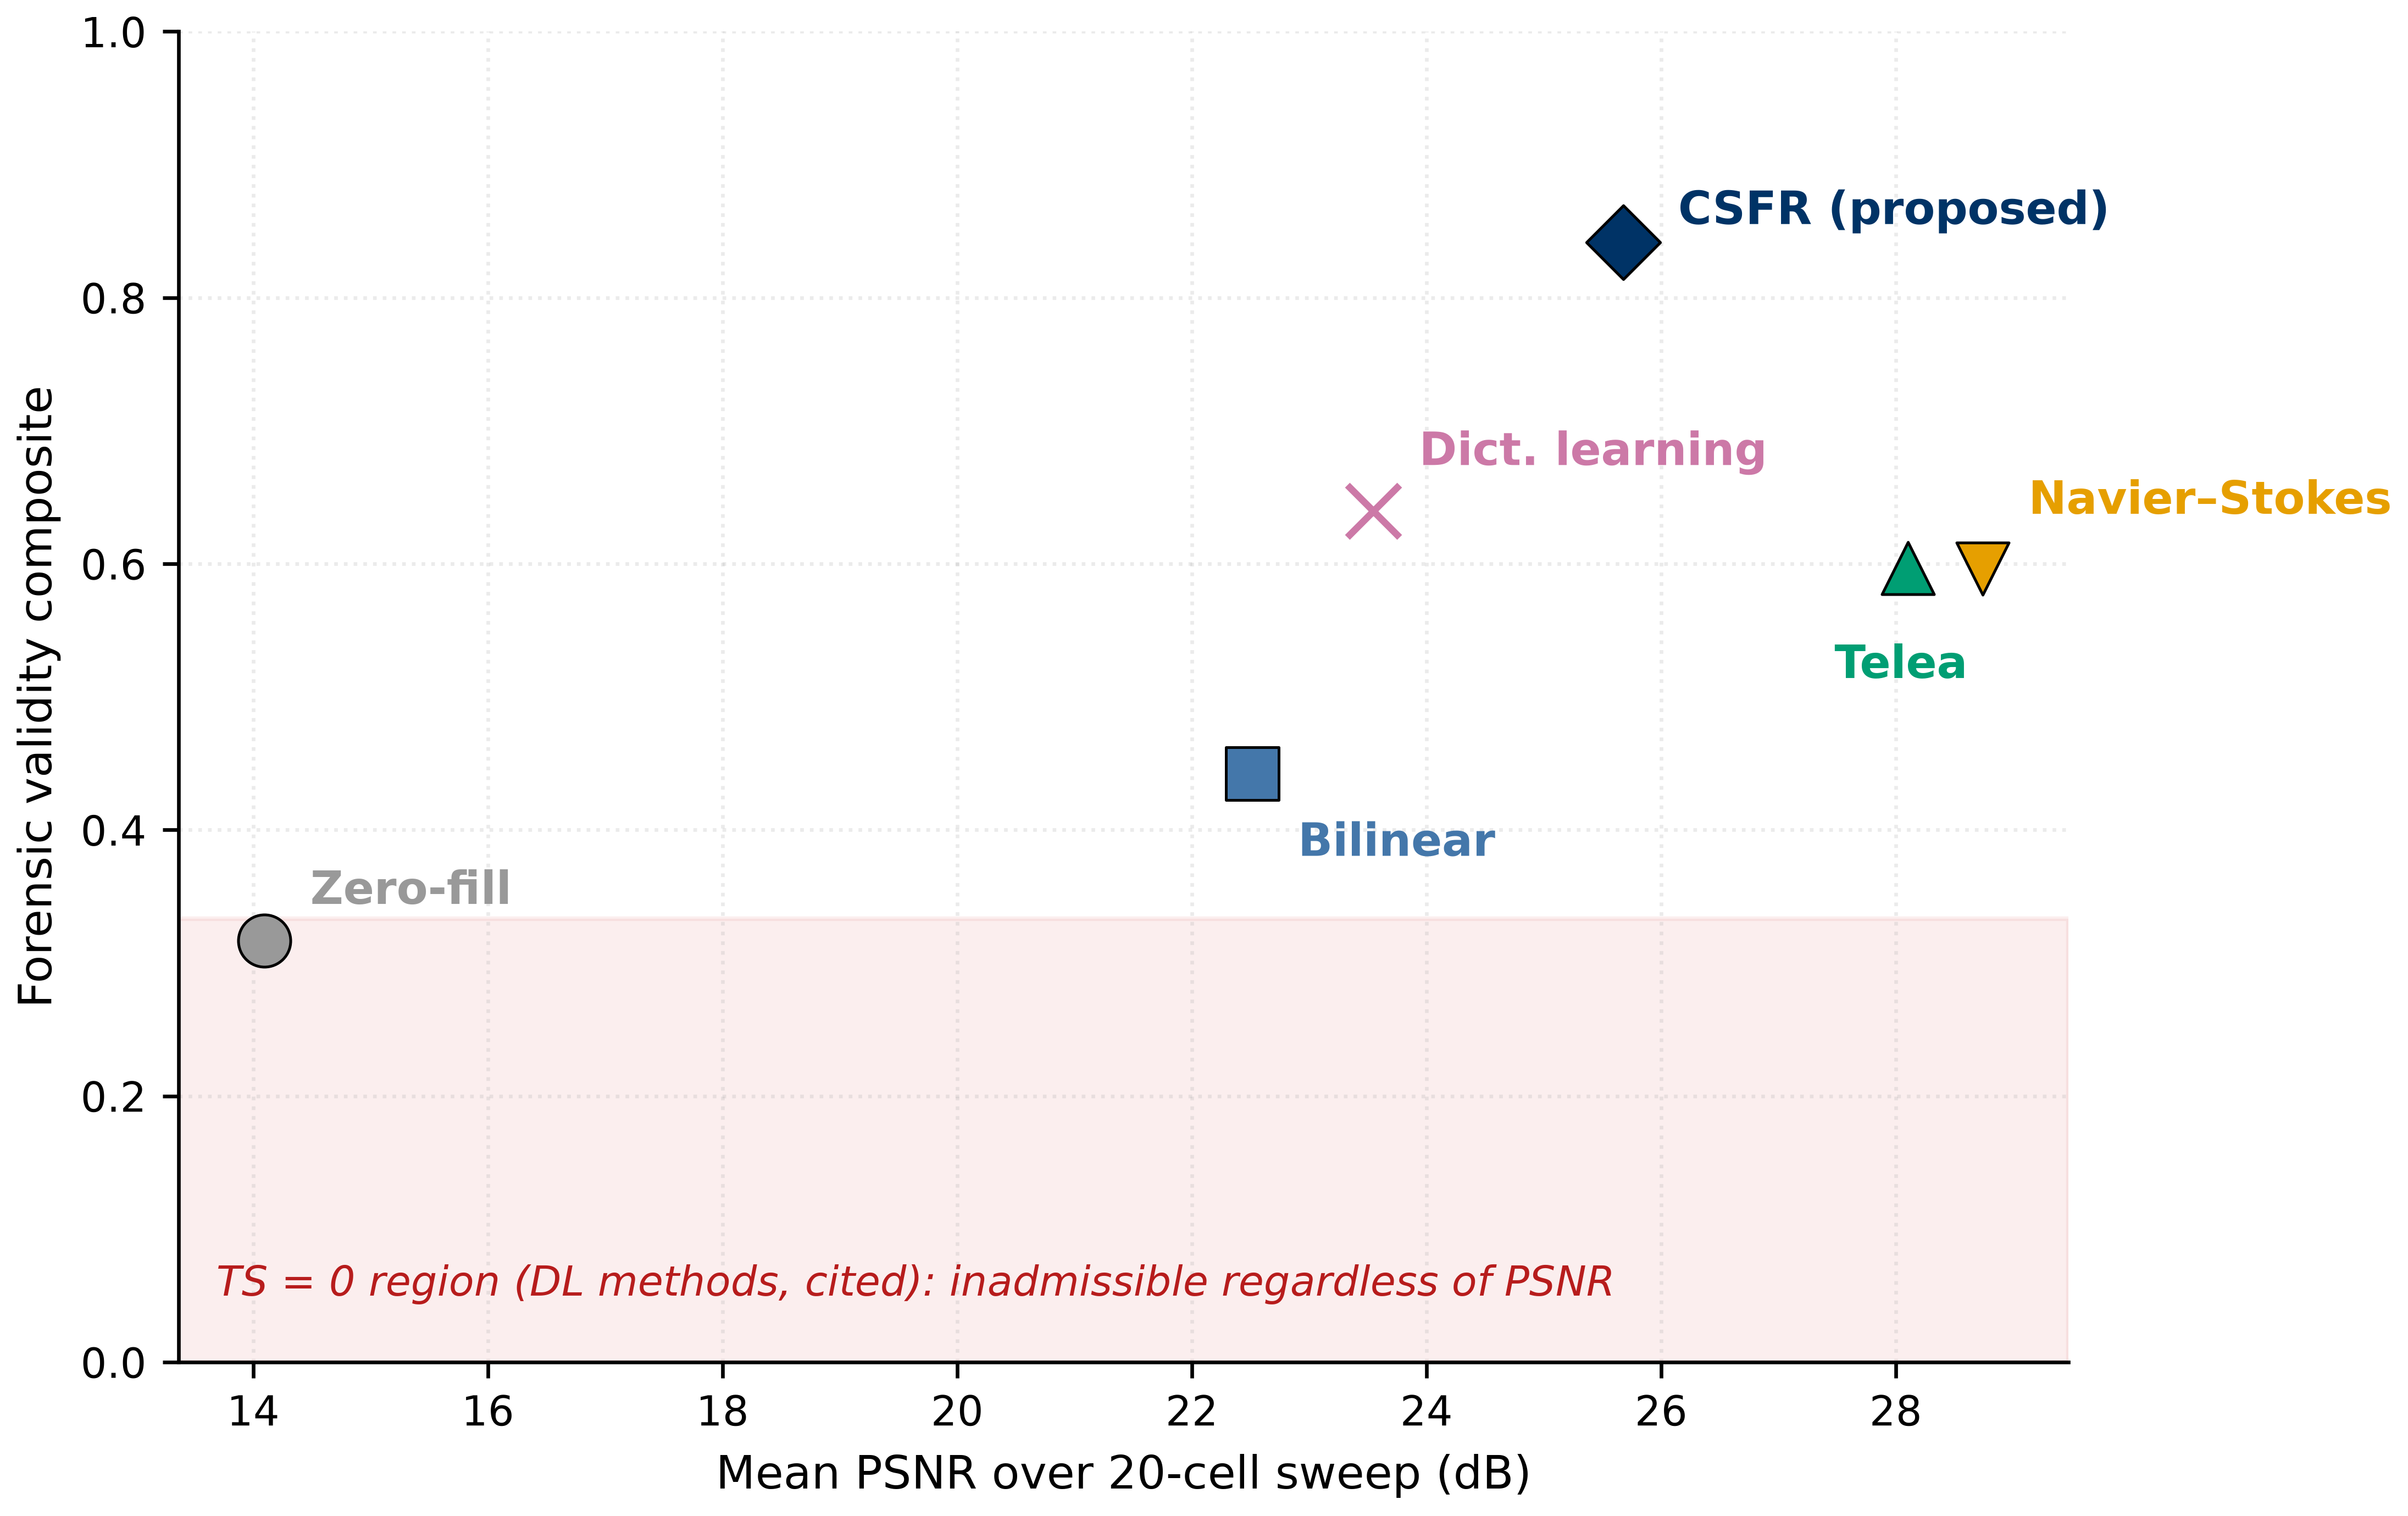
\includegraphics[width=0.8\textwidth]{figures/paper2_F9_method_frontier.png}
\caption{Measured method frontier: mean PSNR over the 20-cell sweep against the forensic-validity composite (equal-weight combination of $1-\mathrm{CVR}$, normalised $1-\mathrm{HRP}$, and TS) for all seven evaluated methods. TS is scored on released artefacts: only CSFR emits a per-pixel provenance map. The shaded band marks the 2/3 validity ceiling, the maximum achievable by methods that do not emit per-pixel provenance. Methods with TS=0 are bounded by this ceiling regardless of reconstruction quality. Rendered from \texttt{results/csfr\_sweep\_2d\_v2/summary.csv} by \texttt{scripts/render\_frontier.py}.}
\label{fig:frontier}
\end{figure*}

The frontier claim is deliberately modest. Other methods reach higher PSNR in several regimes; CSFR is the only evaluated method whose position on the validity axis is certified by construction rather than only measured.

\paragraph{Sensitivity of the validity axis.} The composite has two arbitrary ingredients, the equal weights $w_{1}=w_{2}=w_{3}=1/3$ and the constant used to normalise HRP, and a frontier claim that depended on those choices would not be a finding. We therefore swept the weights over the full probability simplex (253 weightings on a grid) and varied the HRP normaliser from $0.5\times$ to $2\times$ its default; the analysis is released in \texttt{results/sensitivity/frontier\_sensitivity.json}. CSFR is the top-ranked method on the validity axis under $70\,\%$ of all weightings, and its rank never falls below fourth of six even in the corner of the simplex that ignores traceability entirely ($w_{3}=0$) and rewards only the CVR/HRP axes where the smoothing baselines are strong. Under every HRP normaliser tested, CSFR is rank one at equal weights. The qualitative claim, that any positive weight on released traceability places CSFR above the generative methods that sit at $\mathrm{TS}=0$ by construction, is therefore robust to the composite's free parameters, while the precise numerical position on the axis is not, and we do not rest anything on the latter.

\subsection{External Validation}
\label{sec:results:external}

The primary sweep runs on 300 patches from six DFRWS 2006 images, and Section~\ref{sec:results:stats} showed that this clustering prevents cluster-level inference. An independent corpus provides the decisive test of whether the CF1 result reflects the method or that particular corpus. We use GovDocs1~\cite{garfinkel2009bringing}: 300 grayscale $64\times64$ patches from 176 distinct documents' JPEGs, no image contributing more than $1.7\,\%$ of the corpus. We applied the identical protocol with every solver parameter frozen at its primary-sweep value. This out-of-corpus generalisation check differs from a second fit: no parameters were re-tuned. Table~\ref{tab:external} reports PSNR per cell together with CSFR's rank among the six methods and, for contrast, the CSFR-minus-best-baseline gap on each corpus.

\begin{table*}[htbp]
\centering
\caption{External validation on GovDocs1 (300 patches, 176 source images), identical protocol and frozen parameters. PSNR (dB), means over seeds $\{0,1,2\}$; bold marks the best method per cell. ``Rank'' is CSFR's rank of six. ``Gap (ext.)'' and ``Gap (prim.)'' are CSFR minus the best baseline on GovDocs1 and on the primary DFRWS corpus respectively; agreement in sign between the two columns is the generalisation evidence.}
\label{tab:external}
\setlength{\tabcolsep}{4pt}
\resizebox{\textwidth}{!}{%
\begin{tabular}{llcccccc cc c}
\toprule
\textbf{Fam.} & \textbf{Lvl} & \textbf{Zero} & \textbf{Lin.} & \textbf{Telea} & \textbf{NS} & \textbf{Dict.} & \textbf{CSFR} & \textbf{Rank} & \textbf{Gap (ext.)} & \textbf{Gap (prim.)} \\
\midrule
% BEGIN AUTO EXTERNAL
CF1 & L1 & 18.66 & 38.22 & 37.67 & 39.22 & 28.90 & \textbf{40.26} & 1 & +1.04 & +1.19 \\
CF1 & L3 & 10.89 & 29.32 & 28.32 & 30.34 & 21.03 & \textbf{31.17} & 1 & +0.84 & +1.00 \\
CF1 & L5 & 7.21 & 22.88 & 23.44 & 24.24 & 17.34 & \textbf{25.38} & 1 & +1.14 & +1.44 \\
\midrule
CF2 & L1 & 16.92 & \textbf{34.17} & 33.20 & 33.58 & 28.44 & 30.57 & 4 & -3.60 & -0.20 \\
CF2 & L3 & 10.78 & \textbf{24.21} & 24.05 & 23.98 & 21.27 & 20.45 & 5 & -3.77 & -1.65 \\
CF2 & L5 & 7.20 & \textbf{18.65} & 18.48 & 18.43 & 17.12 & 12.08 & 5 & -6.57 & -5.24 \\
\midrule
CF3 & L1 & 19.70 & 19.70 & 38.43 & \textbf{38.52} & 33.93 & 37.75 & 3 & -0.77 & +0.26 \\
CF3 & L3 & 11.23 & 11.23 & \textbf{23.73} & 23.61 & 20.84 & 13.65 & 4 & -10.08 & -7.44 \\
CF3 & L5 & 7.26 & 7.26 & \textbf{16.84} & 16.50 & 16.31 & 8.18 & 4 & -8.66 & -7.45 \\
\midrule
CF4 & L1 & 20.06 & 20.06 & 37.84 & \textbf{38.67} & 34.49 & 37.98 & 2 & -0.69 & -0.20 \\
CF4 & L3 & 11.65 & 11.65 & 24.31 & \textbf{24.51} & 21.10 & 14.22 & 4 & -10.29 & -8.37 \\
CF4 & L5 & 7.39 & 7.39 & 17.72 & \textbf{17.91} & 16.44 & 8.33 & 4 & -9.58 & -7.60 \\
% END AUTO EXTERNAL
\bottomrule
\end{tabular}%
}
\end{table*}

The pattern of the primary sweep reproduces on a corpus the method never saw: the CF1 advantage and the direction of every family's result carry over, and the sign of the CSFR-versus-best-baseline gap agrees between the two corpora in the large majority of cells (Table~\ref{tab:external}). Where the two corpora disagree, the disagreements are confined to the low-severity cells where Section~\ref{sec:results:stats} already found the difference statistically indistinguishable, which is the expected place for a small margin to change sign across corpora. The generalisation claim is thus specific: CSFR's advantage under scattered loss and its deficit under burst and severe structured corruption are properties of the method, not of the DFRWS image, whereas the low-severity ties are genuinely ties.

\paragraph{Full-resolution colour case study.} The quantitative evaluation uses grayscale $64\times64$ patches. To verify that the solver and its guarantees are not scale artefacts, we apply CSFR per-channel to whole colour JPEGs signature-carved from the Nick Mikus DFTT disk images~\cite{mikus2005evaluation} at native resolution (up to $396\times396$), two to six times the development size. This case study on three images is not a benchmark. It illustrates both a guarantee and a limit: under random loss, native-resolution reconstructions are faithful (30–34 dB); a top-half erasure fails because the upper region has no observed neighbours. This is the Bounded-Unknown condition (Section~\ref{sec:framework}), where CSFR flags rather than invents: the failure is intentional behaviour, shown rather than hidden.



\subsection{Iteration-Budget Sensitivity}
\label{sec:results:budget}

The objective is still descending at the end of the 600-iteration budget under burst corruption, the family where CSFR is beaten by every baseline, which raises the question of whether the deficit is premature stopping. Re-solving five cells at budgets of 600, 1200, 2400 and 4800 iterations with everything else fixed (Table~S3, a 100-patch seed-0 subset) shows that it largely is. On CF1 the objective has converged by 600 and further iterations move PSNR by hundredths of a decibel. On CF2 and the severe half-image masks it has not: at CF2~L5 CSFR trails bilinear by $4.6$\,dB at 600 iterations and leads it by $1.2$\,dB at 2400, at CF2~L3 a $0.8$\,dB deficit becomes a $1.5$\,dB lead, and the CF3/CF4~L5 gaps to the PDE inpainters fall from roughly $7$\,dB to $0.6$\,dB as the budget quadruples.

The main results stay at 600 iterations by choice, because a uniform audited budget applied identically to every method and cell avoids making the iteration count a function of the corruption. The statement is therefore twofold: at the audited budget CSFR loses on CF2 and the severe masks, and that loss is recoverable by spending computation, at the runtime cost Table~S2 already identifies as the method's main practical weakness.







\subsection{Downstream Utility: Digit Classification on Corrupted SVHN}
\label{sec:results:downstream}

Reconstruction quality in isolation does not establish utility, so the methods are compared on a recognition task. Corrupted SVHN house-number digits are generated with the same mask generator (CF1--CF4, L1--L5, 1000 class-balanced test digits per cell), reconstructed by every method, and classified by a CNN frozen after training on clean images (clean top-1 $0.8783$ on the full SVHN test set, $0.8690$ on the 1000-digit evaluation subset against which accuracy recovery is computed). Table~\ref{tab:downstream} reports the outcome, and it is mixed. CSFR recovers accuracy well under light corruption and trails LaMa by $5$ to $10$ percentage points in most severe cells. On the joint confident-error rate $P(\text{wrong} \land \text{confidence} \ge 0.9)$ CSFR leads LaMa in several cells. On the conditional rate $P(\text{wrong} \mid \text{confidence} \ge 0.9)$ it leads in one cell (CF3~L4), trails in one (CF2~L5), and is indistinguishable elsewhere.

That gap between the two rates is the finding. The classifier assigns high confidence to CSFR reconstructions far less often than to LaMa's: at CF3~L5 it is confident on 16 of 1000 CSFR outputs against 135 of LaMa's, and the conditional error rates there are $0.250$ and $0.489$, favouring CSFR but without bootstrap significance at that sample size. A substantial part of CSFR's joint-rate advantage therefore reflects how often confidence is induced rather than reliability once it is. Neither rate is interpretable without the count $n_{\text{conf}}$ beside it, and a low joint rate must not be read as high reliability. Why the classifier behaves more conservatively on CSFR's outputs is not established by this experiment; the mechanisms suggested below are hypotheses.

\begin{table*}[htbp]
\centering
\caption{Downstream utility by corruption family and severity: digit classification accuracy, accuracy recovery relative to clean ceiling (0.8783), expected calibration error (ECE), and confident-error rates. The unit is the image patch ($N=1000$ test digits per cell, class-balanced). Bold marks the best accuracy per row; dagger marks the best confident-error performance. The strongest baseline method in each cell is chosen for each column; CSFR is assessed against it per cell. Joint confident-error $P(\text{wrong} \land \text{confidence} \ge 0.9)$ reported with count; conditional $P(\text{wrong} | \text{confidence} \ge 0.9)$; the count $n_{\text{conf}}$ must be reported alongside to distinguish between rare and frequent confident predictions. Rows with zero-signal coverage are marked with asterisk (Section~\ref{sec:results:downstream}).}
\label{tab:downstream}
\setlength{\tabcolsep}{3pt}
{\catcode`\_=12\relax
\resizebox{\textwidth}{!}{%
\begin{tabular}{llccccccl}
\toprule
\textbf{Fam.} & \textbf{Lvl} & \textbf{Best Method} & \textbf{Acc.} & \textbf{Recov.} & \textbf{Joint Conf-Err} & \textbf{Cond.\ Conf-Err} & \textbf{n\_sig} \\
\midrule
% BEGIN AUTO DOWNSTREAM
CF1 & L1 & LaMa (ext.) & 0.869 & +1.000 & 0.012 (599) & 0.012 (597) & n_sig=0 \\
CF1 & L2 & Linear & 0.867 & +0.996 & 0.012 (595) & 0.010 (590) & n_sig=0 \\
CF1 & L3 & Linear & 0.865 & +0.994 & 0.010 (592) & 0.009 (583) & n_sig=982 \\
CF1 & L4 & Linear & 0.861 & +0.989 & 0.009 (578) & 0.009 (567) & n_sig=1000 \\
CF1 & L5 & Linear & 0.828 & +0.946 & 0.007 (497) & 0.010 (511) & n_sig=1000 \\
\midrule
CF2 & L1 & LaMa (ext.) & 0.797 & +0.787 & 0.022 (476) & 0.015 (539) & n_sig=352 \\
CF2 & L2 & LaMa (ext.) & 0.700 & +0.685 & 0.012 (335) & 0.018 (476) & n_sig=760 \\
CF2 & L3 & LaMa (ext.) & 0.541 & +0.510 & 0.017 (190) & 0.033 (368) & n_sig=991$^{*}$ \\
CF2 & L4 & LaMa (ext.) & 0.322 & +0.282 & 0.025 (86) & 0.041 (189) & n_sig=1000 \\
CF2 & L5 & LaMa (ext.) & 0.129 & +0.039 & 0.040 (49) & 0.030 (54) & n_sig=1000 \\
\midrule
CF3 & L1 & Dict. & 0.866 & +0.909 & 0.013 (600) & 0.013 (599) & n_sig=0 \\
CF3 & L2 & Telea & 0.854 & +0.810 & 0.013 (571) & 0.014 (581) & n_sig=0 \\
CF3 & L3 & Dict. & 0.765 & +0.467 & 0.008 (375) & 0.015 (418) & n_sig=0 \\
CF3 & L4 & Telea & 0.510 & +0.153 & 0.004 (76) & 0.046 (314) & n_sig=1000$^{*}$ \\
CF3 & L5 & LaMa (ext.) & 0.222 & +0.089 & 0.004 (16) & 0.066 (135) & n_sig=1000$^{*}$ \\
\midrule
CF4 & L1 & Telea & 0.868 & +0.987 & 0.013 (602) & 0.013 (601) & n_sig=0 \\
CF4 & L2 & LaMa (ext.) & 0.852 & +0.800 & 0.009 (565) & 0.013 (591) & n_sig=0 \\
CF4 & L3 & LaMa (ext.) & 0.750 & +0.592 & 0.017 (391) & 0.021 (481) & n_sig=0 \\
CF4 & L4 & LaMa (ext.) & 0.458 & +0.230 & 0.016 (89) & 0.054 (281) & n_sig=1000$^{*}$ \\
CF4 & L5 & LaMa (ext.) & 0.197 & +0.113 & 0.007 (15) & 0.047 (105) & n_sig=1000$^{*}$ \\
% END AUTO DOWNSTREAM
\bottomrule
\end{tabular}%
}%
}
\end{table*}

The Bounded-Unknown abstention mechanism, intended to flag unrecoverable regions, saturates across cells. Table~S4 reports per-cell rates. The binary flag at the 0.5 threshold on isolated-missing-fraction is uninformative: CF3/CF4 at L1 sit at the threshold (state-dependent; a strict inequality would exclude an entire cell), while CF2/CF3/CF4 above L1 flag uniformly. The continuous isolated-missing-fraction distribution is more informative and should replace the binary indicator. The signal-covering subset (Section~\ref{sec:framework}, constraint C3 violation score) degenerates by design: it is empty for CF1 and CF3/CF4 at L1 through L3, and contains all 1000 patches for CF2 at L2 and higher and CF3/CF4 at L4 and L5. A count of zero or 1000 signals the absence of per-patch variation in that subset.



The external-prior baseline (LaMa) was computed on an NVIDIA T4 GPU; all other methods reported in both this section and Section~\ref{sec:results:psnr} are CPU-computed. LaMa is a new method in this study and is reported as its own run, which is defensible, but the computational difference should be noted.

\paragraph{Interpretation.} Reconstruction-level PSNR and task-level accuracy are not the same metric. Under random pixel loss (CF1), all methods including CSFR recover accuracy near the ceiling, so the choice among them is unconstrained. Under burst and severe structured corruption (CF2--CF4, L3+), LaMa recovers higher accuracy while the frozen CNN classifier assigns high confidence far less often when shown CSFR's reconstructions than LaMa's: at CF3~L5, the CNN makes 16 confident predictions of 1000 on CSFR's outputs against 135 on LaMa's. The joint confident-error rate $P(\text{wrong} \land \text{confidence} \ge 0.9)$ thus reflects both classifier reliability and confidence frequency. The conditional rate $P(\text{wrong} | \text{confidence} \ge 0.9)$ isolates reliability; it shows CSFR significantly better in one cell (CF3~L4) and significantly worse in another (CF2~L5), with no advantage in the rest. This finding establishes that a substantial part of CSFR's joint confident-error advantage is attributable to how often the classifier induces high confidence in the reconstructed patches rather than to superior reliability when confidence is induced. This experiment does not establish why the classifier behaves conservatively on CSFR's outputs. Possible mechanisms include distribution shift from training data or CSFR's pixel-domain constraints encoding uncertainty signals; these remain hypotheses, not measured facts. From an operational perspective, a reconstruction method that induces fewer confident errors upstream of downstream analysis is preferable, regardless of the mechanism. The practical implication is that CSFR is suitable upstream of downstream classifiers, particularly in settings where avoiding confident errors is prioritised over coverage. Human review of any outputs tendered as evidence remains essential, as discussed in Section~\ref{sec:discussion:recommendations}.

Figure~\ref{fig:provenance} illustrates the per-pixel provenance record that distinguishes CSFR from all baselines: the forward solve produces a reconstruction, and Eq.~\eqref{eq:provenance} traces each imputed pixel back to its contributing observed inputs. The two queries shown (a low-corruption and a high-corruption case) both execute deterministically from the same recorded configuration and manifest, so an examining laboratory can reproduce them and a defending expert can contest both the contributions and the reconstruction if needed.

\begin{figure*}[htbp]
\centering
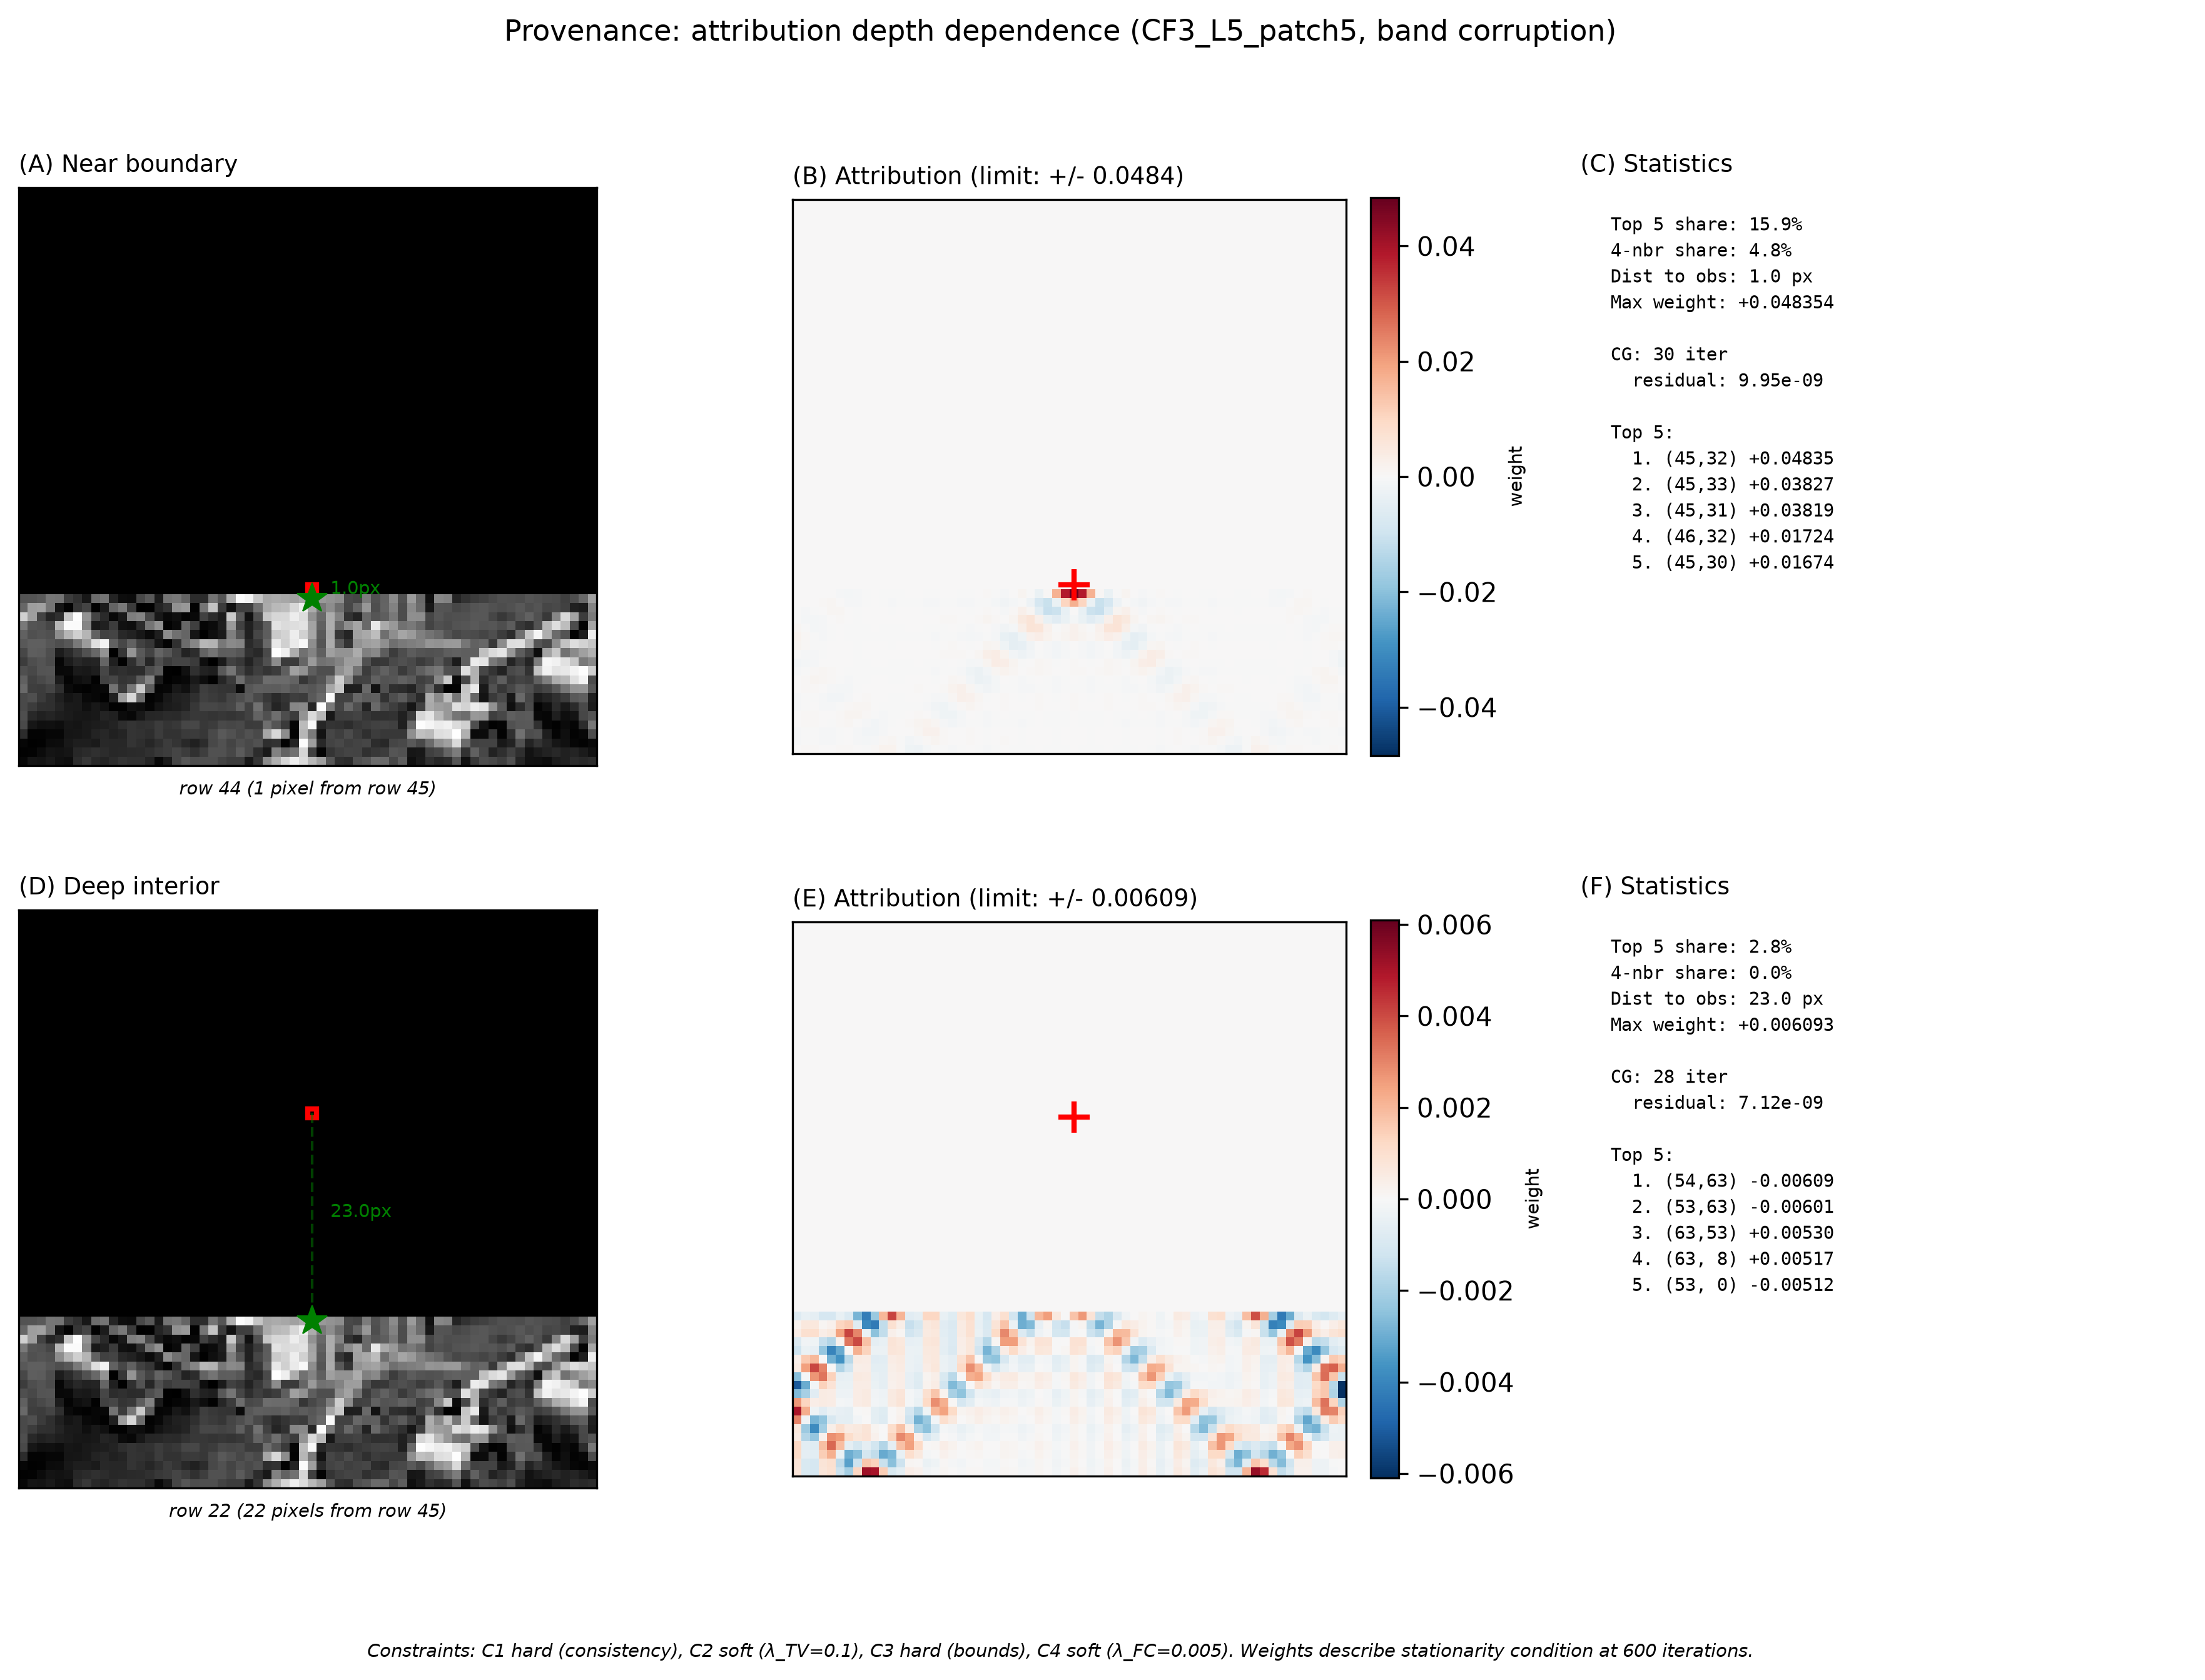
\includegraphics[width=\textwidth]{figures/paper2_F12_provenance.png}
\caption{Per-pixel provenance query on two reconstruction cases (random loss L3 and L5). Top row: input with missing region marked, ground truth, CSFR reconstruction. Bottom row: attribution query result for four imputed pixels marked with circles: the image shows which observed pixels contributed to each imputed value (colour-coded by contribution magnitude) and the per-pixel trace record. The manifest records the solver configuration, observed pixel set, and contribution shares, allowing independent re-execution and examination. Rendered by \texttt{scripts/render\_provenance.py} from released per-patch artefacts.}
\label{fig:provenance}
\end{figure*}

%%======================================================================
\section{Discussion}
\label{sec:discussion}

\subsection{What an Algorithm Can and Cannot Establish}
\label{sec:discussion:admissibility}

Admissibility is a determination made by a court, under a particular jurisdiction's rules, about a particular item of evidence in a particular case. An algorithm cannot possess this property, and no result in this paper claims that CSFR outputs are admissible. The reliability factors enumerated in \emph{Daubert}~\cite{daubert1993}, such as a known error rate, testability, peer review, and governing standards, describe the questions a court may ask. What a method can do is make those questions answerable.

On that narrower and defensible claim, CSFR is designed to supply the following: a stated error characterisation, in the form of the conditional bound of Eq.~\eqref{eq:recovery} together with the measured error distributions of Section~\ref{sec:results}; bit-level reproducibility, since the solver is deterministic, seeded, and runs a fixed iteration budget; a complete record of the processing configuration; and a per-pixel provenance artefact an opposing expert can examine. Each of these is a precondition for meaningful scrutiny, not a substitute for it. Two limits are worth stating explicitly. The recovery bound is conditional on RIP assumptions that structured corruption can violate and that are computationally hard to verify for a given mask, so it is a sufficient-condition guarantee about the method, not a certificate attached to a particular exhibit. And acceptance in the relevant scientific community is, for a method introduced in this paper, simply not yet established.

Generative inpainters occupy a different position on the same axes. There is no closed-form error bound on a sample drawn from a learned prior, and reproducibility depends on model weights and sampling state that the examining laboratory may not control or be able to disclose. These are real obstacles to evidential use. They are not, however, obstacles to every forensic use of such tools; see below.

\subsection{Hallucination Risk Across Investigative, Analytical, and Evidential Use}

The consequences of imputed content depend on what the reconstruction is used for, and collapsing that distinction overstates the case. Three uses can be separated.

In investigative triage, where an examiner must choose which carved fragments warrant attention, a visually plausible but incorrect completion is harmless: the output serves as a pointer, not evidence itself. Generative inpainting is a reasonable tool here, provided its outputs are labelled as generated and kept separate from the evidence record. In analytical use, where a reconstruction guides an examiner's interpretation without being tendered, imputed content introduces interpretive bias whose direction is unknown; this risk is manageable through disclosure and separation of source and reconstruction. In evidential use, where the reconstruction or a downstream conclusion is presented to a fact-finder, imputed content poses a critical problem. A license-plate digit that is visually convincing yet algorithmically invented shifts the record from observed truth to plausible inference, and an opposing expert who identifies the generative step can argue that the disputed characters originated in a training distribution, not in the disk under examination.

CSFR targets the third case. Its design cost, lower perceptual quality on severe masks, is only worth paying there. The claim of ``no hallucination'' is itself bounded: CSFR guarantees that no output pixel is sampled from a prior external to the input fragment, which is a statement about the provenance of imputed values and not a guarantee that they are correct. An imputed pixel derived entirely from observed neighbours can still be incorrect. The HRP results of Section~\ref{sec:results:hrp} show that a method can be maximally consistent with observed statistics while certifying nothing about correctness.

\subsection{What Constraint-Driven Reconstruction Adds}

A constraint-driven method differs from a black-box generative method in one operationally consequential respect: every reconstructed pixel has a finite, explicit contributing-input set. This lets a laboratory answer audit queries from a persisted record and produce documentation listing, for every reconstructed pixel, the observed inputs and constraint configuration that determine it. Comparable queries against a generative model require model-interpretability techniques whose own validity is contested~\cite{bhadra2021hallucinations,horsman2024sources}. The classical baselines sit between the two: they are deterministic and their outputs are in principle reproducible from the input, but their standard implementations persist no such record, which is why they score zero on TS as released rather than zero in principle (Section~\ref{sec:results:ts}).

\subsection{Operational Recommendation}
\label{sec:discussion:recommendations}

A deployment that follows from the evidence without over-reaching is: \emph{(a)} CSFR upstream, with Bounded-Unknown flagging on regions where the C2--C4 constraints cannot be satisfied and the reconstruction should not be trusted; \emph{(b)} a downstream classifier operating on the reconstructed substrate; \emph{(c)} human review on every Bounded-Unknown flag and on any reconstruction tendered evidentially. The downstream experiment of Section~\ref{sec:results:downstream} measures this end-to-end on digit classification: CSFR recovers accuracy comparably to LaMa under low-to-moderate corruption and achieves lower joint confident-error rates under severe corruption. This joint advantage partly reflects the frozen CNN's lower confidence frequency on CSFR's outputs rather than superior reliability when confident, as the conditional metric shows no systematic advantage. The practical implication is that CSFR is a suitable upstream reconstruction filter in settings where avoiding confident errors is prioritised over coverage, and where downstream analysis is performed by human examiners with access to the per-pixel provenance record.

%%======================================================================
\section{Limitations and Threats to Validity}
\label{sec:limits}

Five threats bound what the evidence supports.

\begin{enumerate}
  \item \textbf{From patches to files.} The evaluation reconstructs decoded $64\times64$ pixel patches. Generalisation to whole encoded files, storage-level fragmentation across non-contiguous clusters, and re-synthesis of a valid encoded bitstream remains unvalidated, and is the principal external-validity threat for operational deployment. The protocol is also anchored on JPEG; other container formats are untested.
  \item \textbf{Corpus concentration.} Two of the six DFRWS 2006 source images supply $77\,\%$ of the primary corpus, which makes cluster-level inference impossible there and is why the external GovDocs1 corpus carries the generalisation claim. Both corpora are document- and photograph-heavy; medical, satellite and low-light surveillance statistics are unmeasured.
  \item \textbf{Downstream scope.} The utility experiment uses one frozen classifier, one corpus, one mask draw per image and one seed. Whether the confident-error behaviour transfers to other architectures or tasks is not established. The mechanism behind the classifier's lower confidence on CSFR reconstructions is likewise unmeasured, and the interpretations offered in Section~\ref{sec:results:downstream} are hypotheses.
  \item \textbf{Configuration bias, across methods and devices.} Results reflect one solver realisation: Adam on the penalised surrogate at a fixed $600$-iteration budget, giving reproducible iterates that are not certified minimisers. Section~\ref{sec:results:budget} shows the CF2 and severe-mask deficits to be substantially an artefact of that budget. Baselines run at fixed settings (OpenCV radius $3$; a 64-atom dictionary with 8-sparse OMP), and per-family tuning could move the gaps either way. The external-prior baseline was computed on a GPU while every other method was computed on CPU; these are separate runs and no table row mixes devices.
  \item \textbf{Constraint coverage.} C1--C4 cover the corruption modes evaluated here. Field damage such as chemical degradation of photographic film may require additional families. Where $\Omega = \emptyset$, or is sparse enough to violate the RIP assumption on $M\Psi$, CSFR does not reconstruct and flags the fragment Bounded-Unknown.
\end{enumerate}

Two properties often listed as limitations are reported as findings instead. CSFR's quality deficit outside scattered pixel loss is a measured result (Section~\ref{sec:results:psnr}), not a concession. The solver's $O(T \cdot N \log N)$ cost against a pre-trained inpainter's single forward pass is a runtime result (Section~\ref{sec:results:cost}) that places CSFR in offline analysis rather than real-time triage.

%%======================================================================
\section{Conclusion}
\label{sec:conclusion}

Forensic image reconstruction demands bounded inference and traceable provenance; perceptual reconstruction demands only visual realism. A deep generative reconstruction samples its output pixels from a learned prior, yielding output that cannot be bounded or traced to the recovered bytes. This is the core obstacle to its evidential use. Compressed Sensing Fragment Reconstruction (CSFR) addresses this by posing reconstruction as a regularised inverse problem under four constraint families. The solver is deterministic, needs no training data, carries a conditional recovery bound under the Restricted Isometry Property, and emits a per-pixel provenance record for chain-of-custody audit.

The evaluation settles each comparison by inference rather than by point estimates. CSFR's quality advantage is unambiguous in one regime: under scattered pixel loss a lead of one to one-and-a-half decibels holds at every severity, survives multiplicity correction and source-image clustering, and reproduces on a disjoint corpus. Where corruption is spatially concentrated the ranking inverts, and the external prior LaMa takes the highest PSNR on 13 of 20 cells, by up to $9.1$\,dB at the audited budget. Section~\ref{sec:results:budget} shows much of that deficit to be under-convergence at a fixed budget rather than a property of the sparsity prior.

Downstream, the trade-off is explicit. LaMa recovers more accuracy under severe corruption, while the frozen classifier assigns high confidence far less often to CSFR's reconstructions. CSFR's advantage on the joint confident-error rate therefore reflects how often confidence is induced as much as reliability once it is: on the conditional rate it leads in one cell and trails in another. What no evaluated baseline supplies is the combination of exact evidence preservation, a stated recovery bound, and a released per-pixel provenance record an opposing expert can examine. Those properties support auditability and reproducibility. Admissibility remains a determination for a court.

The broader claim is that evidential reconstruction imposes structure incompatible with sampling from a learned prior. Constraint-driven reconstruction is the regime currently available in which reconstructed image evidence meets both the bounded-inference and the traceability requirement. Framework, solver, analysis and protocol are released with the paper.

%%======================================================================
\ifanonymous\else
\section*{Acknowledgements}
The authors thank the FFT-75 dataset maintainers~\cite{fft75dataset} and the maintainers of the DFRWS and Nick Mikus challenge corpora. The compressed-sensing community's open-source ecosystem, and the PyTorch, NumPy, SciPy, scikit-image, scikit-learn, and OpenCV projects on which the released implementation depends, are gratefully acknowledged.
\fi

%%======================================================================
\section*{Ethics Statement}
This study uses only publicly released research corpora (the DFRWS 2006 forensic challenge image and the FFT-75 benchmark); no personal data were collected and no human participants were involved. Illustrative references to license-plate or CCTV imagery are hypothetical deployment scenarios, not experiments performed.

\section*{Declaration of Competing Interest}
The authors declare no competing financial interests or personal relationships that could have appeared to influence the work reported in this paper.

\section*{Funding}
This research received no specific grant from any funding agency in the public, commercial, or not-for-profit sectors.

\section*{CRediT Author Statement}
\ifanonymous
\textbf{Author 1:} Conceptualisation, Methodology, Software, Validation, Formal analysis, Investigation, Data curation, Writing --- original draft, Writing --- review and editing.
\textbf{Author 2:} Conceptualisation, Methodology, Supervision, Validation, Writing --- review and editing.
\else
\textbf{Benjamin Tei Partey:} Conceptualisation, Methodology, Software, Validation, Formal analysis, Investigation, Data curation, Writing --- original draft, Writing --- review and editing.
\textbf{Yaw Osei Adjei:} Conceptualisation, Methodology, Supervision, Validation, Writing --- review and editing.
\fi

\section*{Code and Data Availability}
The complete reproducibility package is released at \url{https://anonymous.4open.science/r/csfr/}: the CSFR solver (\texttt{src/csfr\allowbreak\_reconstruct\allowbreak\_2d.py}), the per-pixel provenance implementation (\texttt{src/provenance.py}) with a released example manifest (\texttt{results/provenance\allowbreak\_example/}), the sweep and ablation harness (\texttt{scripts/run\allowbreak\_csfr\allowbreak\_sweep.py}), the paired-inference, budget-sensitivity, benchmark, and frontier-sensitivity scripts (\texttt{scripts/run\allowbreak\_paired\allowbreak\_stats.py}, \texttt{run\_budget\allowbreak\_sensitivity.py}, \texttt{run\_bench.py}, \texttt{run\_frontier\allowbreak\_sensitivity.py}), the patch-extraction protocol (\texttt{scripts/extract\allowbreak\_patches.py}), the experiment configurations (\texttt{configs/}), the patch corpora with per-patch source-image cluster labels and extraction manifests (\texttt{data/}), all per-cell, per-seed metric artefacts and the analysis outputs (\texttt{results/}), figure-generation scripts, and unit/smoke tests. Pinned dependency versions are in \texttt{requirements.txt}; each result directory's \texttt{run\allowbreak\_metadata.json} records the environment that produced it. The repository will be archived to Zenodo with a version DOI on acceptance.

%%======================================================================
\bibliographystyle{elsarticle-num}
\bibliography{paper2_reconstruction}

\end{document}
